% Musab A. Alturki
% October 2018
%
%\documentclass[sigconf,timestamp]{acmart}
\documentclass[sigconf,nonacm=true]{acmart}
\fancyhead{}
 
\usepackage{booktabs} % For formal tables

% Copyright
\setcopyright{none}
%\setcopyright{acmcopyright}
%\setcopyright{acmlicensed}
%\setcopyright{rightsretained}
%\setcopyright{usgov}
%\setcopyright{usgovmixed}
%\setcopyright{cagov}
%\setcopyright{cagovmixed}


% DOI
%\acmDOI{10.475/123_4}

% ISBN
%\acmISBN{123-4567-24-567/08/06}

%Conference
%\acmConference[CPS-SPC'18]{ACM Workshop on Cyber-Physical Systems Security \& Privacy}{October 2018}{Toronto, Canada}
%\acmYear{2018}
%\copyrightyear{2018}

% These commands are optional
%\acmBooktitle{Transactions of the ACM Woodstock conference}
%\editor{Jennifer B. Sartor}
%\editor{Theo D'Hondt}
%\editor{Wolfgang De Meuter}

%%% Custom packages
%
%\usepackage{subcaption} % recommended by ACM for subfigures
\usepackage[caption=false,font=small]{subfig}

\usepackage{pgfplots}
\pgfplotsset{width=10cm,compat=1.9}
\usepgfplotslibrary{fillbetween}

%
%\usepackage{pgf-umlsd}
%\usetikzlibrary{shadows,positioning}

\usetikzlibrary{arrows,shadows,positioning}

\usepackage{listings}

\lstset{ 
%  backgroundcolor=\color{white},   % choose the background color; you must add \usepackage{color} or \usepackage{xcolor}; should come as last argument
  basicstyle=\footnotesize\ttfamily,        % the size of the fonts that are used for the code
  breakatwhitespace=false,         % sets if automatic breaks should only happen at whitespace
  breaklines=false,                 % sets automatic line breaking
  captionpos=b,                    % sets the caption-position to bottom
%  commentstyle=\color{mygreen},    % comment style
%  deletekeywords={...},            % if you want to delete keywords from the given language
%  escapeinside={\%*}{*)},          % if you want to add LaTeX within your code
%  extendedchars=true,              % lets you use non-ASCII characters; for 8-bits encodings only, does not work with UTF-8
  frame=single,	                   % adds a frame around the code
  keepspaces=true,                 % keeps spaces in text, useful for keeping indentation of code (possibly needs columns=flexible)
%  keywordstyle=\color{blue},       % keyword style
%  language=maude,                 % the language of the code
%  morekeywords={*,...},            % if you want to add more keywords to the set
  numbers=left,                    % where to put the line-numbers; possible values are (none, left, right)
  numbersep=5pt,                   % how far the line-numbers are from the code
  numberstyle=\tiny\color{gray}, % the style that is used for the line-numbers
  stepnumber=1,                    % the step between two line-numbers. If it's 1, each line will be numbered
  rulecolor=\color{black},         % if not set, the frame-color may be changed on line-breaks within not-black text (e.g. comments (green here))
  showspaces=false,                % show spaces everywhere adding particular underscores; it overrides 'showstringspaces'
  showstringspaces=false,          % underline spaces within strings only
  showtabs=false,                  % show tabs within strings adding particular underscores
%  stringstyle=\color{mymauve},     % string literal style
  tabsize=2,	                   % sets default tabsize to 2 spaces
%  title=\lstname                   % show the filename of files included with \lstinputlisting; also try caption instead of title
}
%
%\usepackage{color}

%%% Custom commands
%
\newcommand{\todo}[1]{\marginpar{\bf\large$[\ast]$}{\sf [#1]}}

\newcommand{\langl}{\begin{picture}(4.5,7)
\put(1.1,2.5){\rotatebox{60}{\line(1,0){5.5}}}
\put(1.1,2.5){\rotatebox{300}{\line(1,0){5.5}}}
\end{picture}}
\newcommand{\rangl}{\begin{picture}(4.5,7)
\put(.9,2.5){\rotatebox{120}{\line(1,0){5.5}}}
\put(.9,2.5){\rotatebox{240}{\line(1,0){5.5}}}
\end{picture}}


\begin{document}
\title[Statistical Model Checking of RANDAO's Resilience Against Pre-computed Reveal Strategies]
{Statistical Model Checking of RANDAO's Resilience Against Pre-computed Reveal Strategies}
%\titlenote{Produces the permission block, and
%  copyright information}
%\subtitle{Extended Abstract}
%\subtitlenote{The full version of the author's guide is available as
%  \texttt{acmart.pdf} document}

%%%
\author{Musab A. Alturki}
%\author{ }
%\authornote{Dr.~Trovato insisted his name be first.}
\orcid{0001-7957-1081}
\affiliation{%
  \institution{Runtime Verification Inc.}
%  \streetaddress{P.O. Box 840}
%  \city{Dhahran, Saudi Arabia}
%  \state{Ohio}
}
\affiliation{%
%  \department{Information and Computer Science Department}
  \institution{King Fahd University of Petroleum and Minerals}
%  \streetaddress{P.O. Box 840}
%  \city{Dhahran, Saudi Arabia}
%  \state{Ohio}
%  \postcode{34464-8044}
}
\email{musab.alturki@runtimeverification.com}

\author{Grigore Ro\c su}
%\author{ }
%\authornote{Dr.~Trovato insisted his name be first.}
%\orcid{0001-7957-1081}
\affiliation{%
  \institution{Runtime Verification, Inc.}
%  \streetaddress{P.O. Box 840}
%  \city{Dhahran, Saudi Arabia}
%  \state{Ohio}
}
\affiliation{%
%  \department{Information and Computer Science Department}
  \institution{University of Illinois at Urbana-Champaign}
%  \streetaddress{P.O. Box 840}
%  \city{Dhahran, Saudi Arabia}
%  \state{Ohio}
%  \postcode{34464-8044}
}
\email{grosu@illinois.edu}

% The default list of authors is too long for headers.
\renewcommand{\shortauthors}{Alturki and Ro\c su}


\begin{abstract}
Decentralized (pseudo-)random number generation (RNG) is a core process of many emerging distributed systems, including perhaps most prominently, the upcoming Ethereum 2.0 (a.k.a. Serenity) protocol. To ensure security and proper operation, the randomness beacon must be unpredictable and hard to manipulate. A commonly accepted implementation scheme for decentralized RNG is a commit-reveal scheme, known as RANDAO, coupled with a reward system that incentivizes successful participation. However, this approach may still be susceptible to look-ahead attacks, in which an attacker (controlling a certain subset of participants) may attempt to pre-compute the outcomes of (possibly many) reveal strategies, and thus may bias the generated random number to his advantage. To formally evaluate resilience of RANDAO against such attacks, we develop a probabilistic model in rewriting logic of the RANDAO scheme (in the context of Serenity), and then apply statistical model checking and quantitative verification algorithms (using \textsc{Maude} and \textsc{PVeStA}) to analyze two different properties that provide different measures of bias that the attacker could potentially achieve using pre-computed strategies. We show through this analysis that unless the attacker is already controlling a sizable portion of validators and is aggressively attempting to maximize the number of last compromised proposers in the proposers list, the expected achievable bias is quite limited. The full specification of the models developed in this work are available online at \url{https://github.com/runtimeverification/rdao-smc}. 
%However, further measures for strengthening RANDAO against this type of attack (e.g. using verifiable delay functions or VDFs) may be necessary if .     
\end{abstract}


%\copyrightyear{2018} 
%\acmYear{2018} 
%\setcopyright{acmcopyright}
%\acmConference[CPS-SPC '18]{2018 Workshop on Cyber-Physical Systems Security and PrivaCy}{October 19, 2018}{Toronto, ON, Canada}
%\acmBooktitle{CPS-SPC '18: 2018 Workshop on Cyber-Physical Systems Security and PrivaCy Oct. 19, 2018, Toronto, ON, Canada}
%\acmPrice{15.00}
%\acmDOI{10.1145/3264888.3264895}
%\acmISBN{978-1-4503-5992-4/18/10}

%\CopyrightYear{2018} 
%\setcopyright{acmcopyright} 
%\conferenceinfo{CPS-SPC '18,}{October 19, 2018, Toronto, ON, Canada}
%\isbn{978-1-4503-5992-4/18/10}\acmPrice{$15.00}
%\doi{https://imsva91-ctp.trendmicro.com:443/wis/clicktime/v1/query?url=https%3a%2f%2fdoi.org%2f10.1145%2f3264888.3264895&umid=1272F148-7316-1905-A8B2-21A2B8EE9BE6&auth=ec34f7633709e8bd85e48c7fc0c92c09c079e558-4b58fbd6a20241a010ea046d5792f330788363a7}

%
% The code below should be generated by the tool at
% http://dl.acm.org/ccs.cfm
% Please copy and paste the code instead of the example below.
%
%\begin{CCSXML}
%<ccs2012>
%<concept>
%<concept_id>10002978.10002986</concept_id>
%<concept_desc>Security and privacy~Formal methods and theory of security</concept_desc>
%<concept_significance>500</concept_significance>
%</concept>
%<concept>
%<concept_id>10002978.10002986.10002990</concept_id>
%<concept_desc>Security and privacy~Logic and verification</concept_desc>
%<concept_significance>500</concept_significance>
%</concept>
%<concept>
%<concept_id>10002978.10002991.10002993</concept_id>
%<concept_desc>Security and privacy~Access control</concept_desc>
%<concept_significance>500</concept_significance>
%</concept>
%<concept>
%<concept_id>10010520.10010553</concept_id>
%<concept_desc>Computer systems organization~Embedded and cyber-physical systems</concept_desc>
%<concept_significance>500</concept_significance>
%</concept>
%<concept>
%<concept_id>10011007.10010940.10010992.10010998.10003791</concept_id>
%<concept_desc>Software and its engineering~Model checking</concept_desc>
%<concept_significance>500</concept_significance>
%</concept>
%</ccs2012>
%\end{CCSXML}
%
%\ccsdesc[500]{Security and privacy~Formal methods and theory of security}
%\ccsdesc[500]{Security and privacy~Logic and verification}
%\ccsdesc[500]{Security and privacy~Access control}
%\ccsdesc[500]{Computer systems organization~Embedded and cyber-physical systems}
%\ccsdesc[500]{Software and its engineering~Model checking}
%
%\keywords{Distance-bounding protocols, Distance fraud, Probabilistic rewriting, Statistical model checking, {\sc Maude}}
%
\settopmatter{printfolios=true}  %%% show page numbers
\maketitle

\section{Introduction}

Decentralized (pseudo-)random number generation (RNG) is a protocol for RNG in which a number of participants collaborate to produce a random number. The participants, who do not necessarily mutually trust each other, collectively provide a randomness beacon that may be used by the participants themselves or made available as an external service for other users. This RNG process is a core process of many emerging distributed autonomous systems, most prominently proof-of-stake (PoS) consensus protocols, which include the upcoming Ethereum 2.0 (a.k.a. Serenity) protocol~\cite{EF:2018,ButerinB:2018}. Unlike \textit{traditional} proof-of-work systems, in which the process of solving cryptographic puzzles inherently provides a good source of entropy that can effectively be used for RNG, PoS systems do not have that and need to explicitly manage a similar process. In a PoS system, the RNG process is essential for managing validators and attestations in the protocol. Furthermore, in the context of the Ethereum protocol, many decentralized applications (dapps) built on top of the platform, which typically manage assets of potentially very high financial value (such as online lotteries), rely fundamentally on having this platform provide a secure randomness beacon for their proper operation.  

To ensure security of such distributed systems, the randomness beacon must be unpredictable and hard to manipulate. A commonly accepted implementation scheme for decentralized RNG is a commit-reveal scheme, known as RANDAO (due to Youcai Qian~\cite{QianQ:2018}), in which participants first make commitments by sharing hash values of seeds, and then, at a later stage, they reveal their seeds, which can then be used for RNG. In a PoS protocol, and in particular in Serenity~\cite{EF:2018}, the scheme is used repeatedly in a sequence of rounds in such a way that the outcome of a round is used as a seed for generating the random number of the following round. Moreover, the scheme is usually coupled with a reward system that incentivizes successful participation and discourages deviations from the protocol. Several other distributed protocols have also adopted this scheme primarily for its simplicity and flexibility.

However, this approach may still be susceptible to \textit{look-ahead} attacks, in which an attacker (controlling a certain subset of participants -- or proposers in the context of a PoS) may choose to refrain from revealing his seed if skipping results in randomness that is more favorable to the attacker. In general, a powerful attacker may attempt to pre-compute the outcomes of (possibly many) reveal strategies, which are sequences of reveal-or-skip decisions, and thus may anticipate the effects of his contribution to the process and bias the generated random number to his advantage. 

While this potential vulnerability is known and has been pointed to in several works in the literature (e.g.~\cite{ButerinB:2018a,ButerinB:2018b,BonehBBBF:2018}), the extent to which it may be exploited by an attacker and how effective the attack could be in an actual system, such as a PoS system like Serenity, have not yet been thoroughly investigated, besides the exploitability arguments made in~\cite{ButerinB:2018a} and \cite{ButerinB:2018b}, which were based on abstract analytical models. While the high-level analysis given there is useful for gaining a foundational understanding of the vulnerability and the potential of the attack, a lower-level formalization that captures the interactions of the different components of the RANDAO process and the environment could provide a more concrete model providing a deeper understanding of the vulnerability and higher confidence in how realizable the attack can be in an actual system. Furthermore, if this formalization is \textit{executable}, it immediately enables quick prototyping and experimentation of different designs, in addition to automating formal reasoning about their exploitability properties, providing a formal tool for guiding the design of a RANDAO scheme or implementation.  

In this work, we develop a computational model of the RANDAO scheme (in the context of Serenity) as a probabilisitic rewrite theory~\cite{KumarKSMA:2003,AghaAMS:2006} in rewriting logic~\cite{MeseguerM:1990} to formally evaluate resilience of RANDAO against pre-computed reveal strategies. The model gives a formal, yet natural, description of (possibly different designs of) the RNG process and the environment. Furthermore, the model is both \textit{timed}, capturing timing of events in the process, and \textit{probabilistic}, modeling randomized protocol behaviors (internal non-determinism introduced by design) and environment uncertainties (external non-determinism induced by, e.g., network delays and failures and colluding behaviors). Being executable, the model allows for generating  random sample executions (Monte Carlo simulations) of the protocol for observing behaviors. Moreover, executability facilitates automated formal analysis of \textit{quantitative properties}, specified as real-valued formulas in \textsc{QuaTEx} (Quantitative Temporal Expressions Logic)~\cite{AghaAMS:2006}, through efficient statistical model checking and quantitative analysis algorithms using both \textsc{Maude}~\cite{ClavelCDELMMT:2007} (a high-performance rewriting system) and \textsc{PVeStA}~\cite{AlturkiAM:2011} (a statistical verification tool that interfaces with \textsc{Maude})\footnote{The reason we chose \textsc{Maude} over $\mathbf{K}$ was because of \textsc{Maude}'s direct support for random number generation and the availability of an interface to \textsc{PVeStA}, which are facilities that are needed for our analysis but not yet available in $\mathbf{K}$.}. Using the model, we analyze two properties that provide different measures of bias that the attacker could potentially achieve using pre-computed strategies: (1) the \textit{matching score}, which is the expected number of proposers that the attacker controls within some time limit, and (2) the \textit{last-word score}, which is the length of the longest tail of the proposers list that the attacker controls within some time limit. %We show through this analysis that although an attacker may be able to bias randomness of the RANDAO scheme, the achievable bias is quite limited, and further measures for strengthening RANDAO against this type of attack (e.g. using verifiable delay functions or VDFs) may not be necessary.

%Although the obtained guarantees are up to some statistical confidence (specified by the user as verification parameters), this method provides an efficient and automatic means of verifying complex systems while avoiding: (1) the notorious state space explosion problem, to which standard dynamic verification methods are vulnerable, and (2) having to make simplifying assumptions that are usually needed for full (or manual) symbolic analysis to be tractable. 

We show through this analysis that unless the attacker is already controlling a sizable portion of validators and is aggressively attempting to maximize the number of last compromised proposers in the proposers list, or what we call the longest \textit{compromised tail} of the list, the expected achievable bias of randomness of the RANDAO scheme is quite limited. Keeping in mind that when skipping a reveal the attacker forfeits the block reward for his turn in the block proposal process, even this limited bias comes at a cost to the attacker, which may render the attack economically infeasible. However, an aggressive attacker who can afford to make repeated skips for very extended periods of time (e.g. in thousands of rounds), or an attacker who already controls a fairly large percentage (e.g. more than 30\%) of participants in the network will have higher chances of success. Therefore, in these cases, further measures for strengthening RANDAO against this type of attack (e.g. using verifiable delay functions or VDFs~\cite{BonehBBBF:2018}) may be necessary.     

The full specifications of the models developed in this work are available online at \url{https://github.com/runtimeverification/rdao-smc}. 
%and at \url{https://github.com/runtimeverification/rdao-smc-minimal}. Both repositories 
The repository includes amply documented specifications, instructions for installing the required tools, and scripts for running the verification tasks described in this report.

The rest of the report is organized as follows. In Section~\ref{sec:rwl}, we review some preliminaries on rewriting logic, \textsc{Maude} and \textsc{PVeStA}. In Section~\ref{sec:randao}, we introduce in some detail the RANDAO scheme. This is followed in Section~\ref{sec:rdao-rwl} by a detailed description of the rewrite theory giving a model of RANDAO in rewriting logic. Section~\ref{sec:rdao-smc} describes the analysis properties and discusses the analysis results. The report concludes with a summary and discussion of future work in Section~\ref{sec:concl}.





\section{Preliminaries}
\label{sec:rwl}

Rewriting Logic~\cite{MeseguerM:1992} is a general logical and semantic framework in which systems can be formally specified and analyzed. A unit of specification in Rewriting Logic is a \emph{rewrite theory} $\mathcal{R}$, which formally describes a concurrent system including its static structure and dynamic behavior. It is a tuple $(\Sigma, E \cup A, R)$ consisting of: (1) a membership equational logic (MEL)~\cite{MeseguerM:1998} signature $\Sigma$ that declares the kinds, sorts and operators to be used in the specification; (2) a set $E$ of $\Sigma$-sentences, which are universally quantified Horn clauses with atoms that are either equations $(t = t')$ or memberships $(t : s)$; (3) $A$ a set of equational axioms, such as commutativity, associativity and/or identity axioms; and (4) a set $R$ of rewrite rules specifying the computational behavior of the system. A rewrite rule has the following form:
\[
(\forall \overrightarrow{x})\; r : t(\overrightarrow{x}) \longrightarrow t'(\overrightarrow{x}) ~ \textrm{if}~ C(\overrightarrow{x})
\]
where $r$ is a label, and $C$ is a conjunction of equational or rewrite conditions. Operationally, if there exists a substitution $\theta$ such that $\theta(t)$ matches a subterm $s$ in the state of the system, and $\theta(C)$ is satisfied, then $s$ may rewrite to $\theta(t')$. While the MEL sub-theory $(\Sigma , E \cup A)$ specifies the user-defined syntax and equational axioms defining the system's state structure, a rewrite rule in $R$ specifies a \textit{parametric transition}, where each instantiation of the rule's variables that satisfies its conditions yields an actual transition, which can happen concurrently with other non-overlapping transitions (See \cite{BruniBM:2006} for a detailed account of generalized rewrite theories). 

\emph{Probabilistic rewrite theories} extend regular rewrite theories with probabilistic rules~\cite{SenSKMA:2003,AghaAMS:2006}. Assuming $\overrightarrow{x}$ and $\overrightarrow{y}$ are disjoint, a probabilistic rewrite rule is of the following form:
\[
(\forall \overrightarrow{x}, \overrightarrow{y})\; r : t(\overrightarrow{x}) \longrightarrow t'(\overrightarrow{x},\overrightarrow{y}) ~ \textrm{if}~ C(\overrightarrow{x}) \; \textrm{with probability} \; \overrightarrow{y} := \pi(\overrightarrow{x})
\]
A probabilistic rule introduces on its right-hand-side term new variables $\overrightarrow{y}$, the values of which depend on a probability distribution function $\pi$ parametrized by $\theta(\overrightarrow{x})$, where $\theta$ is a matching substitution satisfying the condition $C$. %Assuming $\overrightarrow{x}$ and $\overrightarrow{y}$ are disjoint, a probabilistic rewrite rule has the following form:
%\begin{multline*}
%(\forall \overrightarrow{x}, \overrightarrow{y})\; 
%r : t(\overrightarrow{x}) \longrightarrow t'(\overrightarrow{x},\overrightarrow{y}) ~ \textrm{if}~ C(\overrightarrow{x}) \\ \textrm{with probability} \; \overrightarrow{y} := \pi(\overrightarrow{x})
%\end{multline*}
%A probabilistic rule introduces on its right-hand-side term new variables $\overrightarrow{y}$, the values of which depend on a probability distribution function $\pi$ parametrized by $\theta(\overrightarrow{x})$, where $\theta$ is a matching substitution satisfying the condition $C$. 
A canonical example is the probabilistic rule specifying a battery-operated clock~\cite{ClavelCDELMMT:2007}:
\begin{equation*}
\begin{split}
\mathit{clock}(t,c) \longrightarrow \; 
	& \mathbf{if} \; B \;\mathbf{then}\; \mathit{clock}(t + 1, c - c / 1000.0) \\ 
	& \mathbf{else} \;  \mathit{broken} \\ 
	& \textrm{with probability}\; B := \mathit{Bernoulli}(c / 1000.0)
\end{split}
\end{equation*}
%%As the clock $\mathit{clock}(t,c)$ ticks ($t$ is the current time and $c$ is the remaining battery charge), its battery charge decreases, and its chances of transitioning into a $\mathit{broken}$ state increase (controlled by the outcome $B$ of a Bernoulli trial).  
The rule specifies how a clock transitions to its next state, which is either a regular operational state $\mathit{clock}(T,C)$, with $T$ the current time and $C$ the current battery charge, or a broken state $\mathit{broken}$. As the clock ticks, its battery charge decreases. Whether the clock transitions to an operational or a broken state depends on the outcome of a Bernoulli trial with success probability of $C / 1000.0$ used by the new variable $B$. Since the probability of success in a Bernoulli trial is proportional to the current battery charge, the clock will have a higher chance of failing as time elapses and the battery charge decreases.
Probabilistic rewrite theories unify many different probabilistic models and can express systems involving both probabilistic and nondeterministic features. A more detailed account of probabilistic rewrite theories can be found in~\cite{KumarKSMA:2003,SenSKMA:2003}.

\textsc{Maude}~\cite{ClavelCDELMMT:2007} is a high-performance rewriting logic implementation. An equational theory $(\Sigma, E \cup A)$ is specified in \textsc{Maude} as a functional module delimited by \verb+fmod ... endfm+ keywords. A functional module may consist of module inclusion statements for importing other modules (e.g. \verb+protecting MODULEX+), sort and subsort declarations for defining type hierarchies (e.g. \verb+sort Nat+ and \verb+subsort Nat < Int+), operator declarations with the \verb+op+ keyword, and unconditional and conditional equations (with \verb+eq+ and \verb+ceq+ respectively) and memberships (\verb+mb+ and \verb+cmb+). Operator declarations specify the operator's syntax (in mixfix notation), the number and sorts of the arguments and the sort of its resulting expression. Furthermore, equational attributes such as associativity and commutativity axioms may be specified in brackets after declaring the input and output sorts. For example, the following declares constructors for natural numbers (in Peano notation) and the \verb#+# operator, and then defines addition using two equations:
\begin{lstlisting}
op zero : -> Nat [ctor].
op s_   : Nat -> Nat [ctor].
op _+_  : Nat Nat -> Nat [assoc comm] .
eq zero    + N:Nat = N:Nat .
eq s N:Nat + M:Nat = s (N:Nat + M:Nat) .
\end{lstlisting}
The constructor \verb+s_+ is called the \textit{successor} function and is used heavily in specifications in \textsc{Maude} to specify patterns on natural numbers (like the ones used in the definition of the plus operator above). In addition to Peano numbers, \textsc{Maude} includes the standard (decimal) representation of numbers for performance reasons.

A rewrite theory is specified as a \textit{system module} delimited by \verb+mod+ and \verb+endm+ keywords, which may additionally contain rewrite rules declared with the \verb+rl+ keyword (\verb+crl+ for conditional rules). For instance, in a specification of the Wolf-Sheep-Cabbage puzzle, in which the state is represented by a set \verb+S+ (constructed by an associative and commutative empty juxtaposition operator) of objects \verb+E+ , and in which the two sides of the river are modeled by the (ordered) pair \verb+{S:S'}+, a valid move may be modeled by the following conditional rewrite rule:
\begin{lstlisting}
crl [moveRight] : { man E S : S'} => { S : man E S'} 
    if isSafe(S) .
\end{lstlisting}
which states that the man may cross the river with an object \verb+E+ to the right side only if it is safe to leave objects in \verb+S+ on their own on the left side of the river (e.g. \verb+isSafe(wolf sheep)+ is false). 

Furthermore, probabilistic rewrite theories, specified as system modules in \textsc{Maude}~\cite{ClavelCDELMMT:2007}, can be simulated by sampling from probability distributions. 
%This is achieved using \textsc{Maude}'s pseudo-random number generator function \texttt{random(s)}, with \texttt{s} a seed, and a constant \texttt{counter} that rewrites to the next natural number using an internal strategy. 
Using \textsc{PVeStA}~\cite{AlturkiAM:2011}, randomized simulations generated in this fashion can be used to statistically model check quantitative properties of the system. These properties are specified in a rich, quantitative temporal logic, \textsc{QuaTEx}~\cite{AghaAMS:2006}, in which real-valued state and path functions are used instead of boolean state and path predicates to quantitatively specify properties about probabilistic models. \textsc{QuaTEx} supports parameterized recursive function declarations, a standard conditional construct, and a \textit{next} modal operator $\bigcirc$, allowing for an expressive language for real-valued temporal properties (Example \textsc{QuaTEx} expressions appear in Section~\ref{sec:rdao-smc}). Given a \textsc{QuaTEx} path expression and a \textsc{Maude} module specifying a probabilistic rewrite theory, statistical quantitative analysis is performed by estimating the \textit{expected value} of the path expression against computation paths obtained by Monte Carlo simulations. More details can be found in~\cite{AghaAMS:2006}. For more on \textsc{Maude}, the reader is referred to the \textsc{Maude} book~\cite{ClavelCDELMMT:2007}.



\section{The RANDAO Scheme}
\label{sec:randao}

The RANDAO scheme~\cite{QianQ:2018} is a commit-reveal scheme consisting of two stages: (1) the commit stage, in which a participant $p_i$ first commits to a seed $s_i$ (by announcing the hash of the seed $h_{s_i}$), and then (2) the reveal stage, in which the participant $p_i$ reveals the seed $s_i$. The sequence of revealed seeds $s_0, s_1, \cdots, s_{n-1}$ (assuming $n$ participants) are then used to compute a new seed $s$ (e.g. by taking the XOR of all $s_i$), which is then used to generate a random number.  

In the context of the Serenity protocol~\cite{EF:2018}, the RANDAO scheme proceeds in rounds corresponding to epochs in the protocol. At the start of an epoch $i$, the random number $r_{i-1}$ generated in the previous round (in epoch $i - 1$) is used for sampling from a large set of validators participating in the protocol an ordered list of block proposers $p_0, p_1, \cdots p_{k-1}$, where $k$ is the cycle length of the protocol (a fixed number of time slots constituting one epoch in the protocol). Each proposer $p_i$ is assigned the time slot $i$ of the current round (epoch). During time slot $i$, the proposer $p_i$ is expected to submit the pair $(c_{p_i}, s_{p_i})$, with $c_{p_i}$ a commitment on a seed to be used for the next participation in the game (in some future round when $p_i$ is selected again as a proposer), and $s_{p_i}$ the seed to which $p_i$ had previously committed in the last participation in the game (or when $p_i$ first joined the protocol's validator set). The RANDAO contract keeps track of successful reveals in the game, which are those reveals that arrive in time and that pass the commitment verification step. Towards the end of an epoch $i$, the RANDAO contract combines the revealed seeds in this round by computing their XOR $s_i$, which is used as the seed for the next random number $r_{i+1}$ to be used in the next round $i+1$. To discourage deviations from the protocol and encourage proper participation, the RANDAO contract penalizes proposers who did not successfully reveal (by discounting their Ether deposits) and rewards those proposers who have been able to successfully reveal their seeds (by distributing dividends in Ether).   

An important variation of this specification is for a validator $v_i$ to commit (at the time of registration) to a hash onion of the form $H^m(s_i) = H(H( \cdots (s_i) \cdots ))$ ($m$ times), where $m$ is the maximum number of participations in the protocol. Each time $v_i$ is selected to participate in the game (selected as a proposer), the validator $v_i$ reveals a pre-image of the hash onion $H^{m-k}(s_i)$, assuming $v_i$ has already participated $k < m$ times since registration. 

In the analysis below, we chose to model the scheme with commit-reveal pairs above (rather than hash onions) since its simpler and does not require fixing a priori the number of participations of a validator in the RANDAO process. The analysis results, however, apply equally to the hash-onions-based variation of the scheme since the use of hash onions does not affect an attacker's ability to pre-compute reveal strategies. 
 


\section{A Rewriting Model of RANDAO}
\label{sec:rdao-rwl}

We use Rewriting Logic~\cite{MeseguerM:1992}, and its probabilistic extensions~\cite{KumarKSMA:2003,AghaAMS:2006}, to build a generic and executable model of the RANDAO scheme. The model captures at a high level of abstraction the essential structural and behavioral aspects of a RANDAO process. Furthermore, using \textsc{Maude}~\cite{ClavelCDELMMT:2007}, the model can be simulated to generate random sample executions that can be used to statistically model-check probabilistic properties of the protocol, including resilience against look-ahead attacks using pre-computed reveal strategies. In this section, we describe the model and its behaviors in some detail. %The full specification of the model in \textsc{Maude} is available online at \url{https://github.com/runtimeverification/rdao-smc}. 

\subsection{The Rewrite Theory $\mathcal{R}$ of RANDAO}

We introduce a model of RANDAO as a probabilistic rewrite theory $\mathcal{R} = (\Sigma_\mathcal{R}, E_\mathcal{R} \cup A_\mathcal{R}, R_\mathcal{R})$ specified in \textsc{Maude} as a system module. The full \textsc{Maude} specification is available online at \url{https://github.com/runtimeverification/rdao-smc}. By utilizing different facilities provided by its underlying formalism, the model $\mathcal{R}$ is both \textit{probabilistic}, specifying randomized behaviors and environment uncertainties, and \textit{real-time}, capturing time clocks and message transmission delays. Furthermore, the model is \textit{parametric} to a number of parameters, such as the attack probability, the size of the validator set and the network latency, among others (there are 11 parameters in total, discussed in Section~\ref{sec:params}), to enable capturing different scenarios and attack behaviors. 

\subsection{Model Infrastructure}
\label{sec:infra}
We begin by describing fundamental data types and operations that are used throughout the model. These components are specified by the MEL sub-theory $(\Sigma_\mathcal{R}, E_\mathcal{R} \cup A_\mathcal{R})$ of $\mathcal{R}$.

\textbf{Seeds and hashes.} We represent seeds as arbitrary positive integers (of type \textsf{NzNat} for non-zero natural numbers). For computational efficiency, however, we limit the allowed values as seeds to \texttt{\#MAX-SEED-VALUE}, which is taken as the largest random value that can be produced by \textsc{Maude}'s \texttt{random} operator\footnote{The potential inefficiency is due to \textsc{Maude}'s implementation of the random function being based on the Mersenne Twister RNG (in
which computing the random value corresponding to S requires computing the previous value for S-1), which was not designed to support arbitrary, user-supplied seeds.}. The hash function is abstractly represented by the hash (constructor) operator:
\begin{lstlisting}
op h : Seed -> Hash [ctor frozen] .
\end{lstlisting}  
with \textsf{Seed} the sort of seed values, and \textsf{Hash} the sort of hashed values. The operations of committing to a seed \texttt{S} and revealing a committed seed \texttt{h(S)} are defined as expected:
\begin{lstlisting}
op commit : Seed -> Hash .   eq commit(S) = h(S) .
op reveal : Hash -> Seed .   eq reveal(h(S)) = S .  
\end{lstlisting}  
A basic operation in RANDAO is computing the XOR of the current seed maintained by the contract \texttt{S} and the recently revealed seed \texttt{S'} by a proposer, which is captured by the following operation:
\begin{lstlisting}
op combineSeeds : Seed Seed -> [Seed] .
eq combineSeeds(S, S') = (S xor S') rem #MAX-SEED-VALUE .
\end{lstlisting}  
As explained above, the new seed is assumed not to exceed the value of \texttt{\#MAX-SEED-VALUE} (a large value) for execution efficiency, which is enforced using the remainder \verb+rem+ operation. 


\textbf{Index lists and sets.} As validators in the system will be identified by their indices (of sort \textsf{Nat} for natural numbers), the model will need to manipulate lists of validators, which are naturally represented by lists of their indices. We therefore define the sort \textsf{NatList} as a super-sort of \textsf{Nat}, so that a natural number is itself a (singleton) list, that is constructed by an associative binary dot operator with identity \texttt{nilIL}:
\begin{lstlisting}
op nilIL : -> NatList [ctor] .
op _._ : NatList NatList -> NatList [ctor assoc id: nilIL] .
\end{lstlisting}  
Since seeds are also natural numbers, we note that a \textsf{NatList} term can have different interpretations depending on the context. For example, the term \texttt{ 748 . 42 . 908 } can be interpreted as a list of three validators identified by the indices 748, 42 and 908, or as a list of three seed values. Throughout the report, we will assume that a \textsf{NatList} term represents a list of validator indices, unless indicated otherwise. 

Furthermore, it will be convenient to manage collections of indices as sets. For that we construct a set of indices (of the sort  \textsf{NatSet}, declared as a super-sort of \textsf{Nat}) using and associative, commutative and idempotent comma operator with identity \texttt{mtIS}.
\begin{lstlisting}
op mtIS : -> NatSet [ctor] .
op _,_ : NatSet NatSet -> NatSet 
            [ctor assoc comm id: mtIS] .
eq I , I = I .
\end{lstlisting}  

In addition to the basic operations of \textsf{length(IL)} (returning the length of an index list \textsf{IL}) and \textsf{toNatSet(IL)} (mapping an index list to its corresponding index set), there are three foundational operations that we define on the sort \textsf{NatList} (as validator lists). The operator \texttt{sampleIndexList(N,K,S,IL)} specifies a function that computes a new list of validators (as proposers) of length \verb+K+ with no repeated validators, given a seed \verb+S+ and the size of the entire validator set \verb+N+ as input parameters: 
\begin{lstlisting}
 op sampleIndexList : Nat Nat Seed NatList -> [NatList] .
 eq sampleIndexList(N, 0, S, IL) = IL .
ceq sampleIndexList(N, s(K), S, IL) 
   = sampleIndexList(N, K, S, IL . M) 
   if M := 
   computeUniqueIndex(N, (S * s(K) * s(s(K))) rem N, IL) .
\end{lstlisting}  
This definition uses an auxiliary operator \verb+computeUniqueIndex+ that returns an index that does not appear in the given list of already sampled indices:
\begin{lstlisting}
op computeUniqueIndex : Nat Nat NatList -> [Nat] .
eq computeUniqueIndex(N, M, IL . M . IL') 
  = computeUniqueIndex(N, s(M) rem N, IL . M . IL') .
eq computeUniqueIndex(N, M, IL) = M [owise] . 
\end{lstlisting}  
If the computed index \verb+M+ already appears in the list \verb+IL+, then the next index \verb+s(M)+ is attempted and the check is recursively repeated. Otherwise, the index \verb+M+ is returned. This enforces the requirement that a proposer cannot appear repeated in the proposers list of a given round. 

We note that in an actual implementation of the system, the seed S would be used as input to a pseudo-random number generator to sample the list of indices. This is not done here, as it might result in an inefficient specification. Instead, we generate our pseudo-random number using an arithmetic combination of the seed S and the position in the list for which the number is being generated. It is important to note that this approach is still faithful to the original protocol since the seed S itself is generated pseudo-randomly (using the function \verb+random+), and thus, the resulting number is also pseudo-random. For example, the expression \texttt{sampleIndexList(100,5,748692,nilIL)} returns the ordered sample of size 5 from the set of indices $\{0, \dots, 99\}$ computed using the seed 748692, which is \verb+ 60 . 40 . 4 . 52 . 84+.

The other two operators on \textsf{NatList}, namely \texttt{countCompromised} and \texttt{countCompromisedTail}, specify functions that count the number of indices in a list that satisfy certain conditions. The expression \texttt{countCompromised(L1, L2)} returns the number of indices in the first list \texttt{L1} that appear in the second list \texttt{L2}. Therefore, if \texttt{L1} represents the list of proposers and \texttt{L2} is a list of all compromised validators, the expression gives the number of compromised proposers in the current round, which is one important measure of the success of an attack, as we will see later. This operation is defined using an auxiliary (tail-recursive) operator \texttt{countCompromised*(L1, L2, N)}, which uses matching (modulo associativity and identity) to count matching indices and maintains that count in \texttt{N}:
\begin{lstlisting}
op countCompromised : NatList NatList -> [Nat] .
eq countCompromised(IL1, IL2) 
  = countCompromised*(IL1, IL2, 0) .

op countCompromised* : NatList NatList Nat -> [Nat] .
eq countCompromised*((IL1 . I . IL1'),(IL2 . I . IL2'), N)
  = countCompromised*((IL1 . IL1'),(IL2 . I . IL2'), s(N)) .
eq countCompromised*(IL1, IL2, N) = N [owise] .
\end{lstlisting}  

For the second operator, the expression \texttt{countCompromisedTail(L1, L2)} returns the number of indices comprising the longest tail of \texttt{L1} that appear in \texttt{L2}. When \texttt{L1} is the list of proposers and \texttt{L2} is the list of attacker-controlled validators, the function computes the length of the longest \textit{compromised tail} of \texttt{L1}. In its definition, this operator similarly uses another auxiliary (tail-recursive) operator \texttt{countCompromisedTail*(L1, L2, N)}, which again uses matching (modulo associativity and identity) to count matching indices and maintains that count in \texttt{N}:
\begin{lstlisting}
op countCompromisedTail : NatList NatList -> [Nat] .
eq countCompromisedTail(IL1, IL2) 
  = countCompromisedTail*(IL1, IL2, 0) .

op countCompromisedTail* : NatList NatList Nat -> [Nat] .
eq countCompromisedTail*((IL1 . I), (IL2 . I . IL2'), N)
  = countCompromisedTail*(IL1, (IL2 . I . IL2'), s(N)) .
eq countCompromisedTail*(IL1, IL2, N) = N [owise] .
\end{lstlisting}  
   
In addition to the operators above, we further define a \textit{selector} operation \texttt{computeScoreFunction(N, L1, L2)} which returns the number of compromised proposers given by \texttt{countCompromised(L1, L2)} if \verb+N+ is 0, or the length of the longest compromised tail given by \texttt{countCompromisedTail(L1, L2)} if \verb+N+ is 1. 
\begin{lstlisting}
op computeScoreFunction : Nat NatList NatList -> [Nat] .
eq computeScoreFunction(0, IL, IL') 
  = countCompromised(IL, IL') .
eq computeScoreFunction(1, IL, IL') 
  = countCompromisedTail(IL, IL') .
\end{lstlisting}  
This selection operation will be useful for modularly defining the function for which the attacker is trying to optimize.   

\textbf{Validator roles.} A validator participating in the system is either an honest validator that is following the protocol or a compromised validator that is controlled by the attacker (which may not necessarily follow the protocol). When selected as a proposer, a compromised validator may behave differently from other compromised validators depending on its position in the proposers list. To distinguish these possible behaviors, we identify three possible roles of a compromised validator selected as a proposer: (1) \texttt{isolated}, which is a compromised proposer that does not belong to a compromised tail of the proposers list (recall that a compromised tail of a list $L$ is a suffix of $L$ consisting entirely of compromised validators), (2) \texttt{ctailhead}, which is the compromised proposer that is positioned at the head of the longest compromised tail of the list, and (3) \texttt{ctailtail}, which is a compromised tail proposer other than the head identified by the role \texttt{ctailhead}. For example, if we assume that the validators indexed by 1, 3, 5 and 7 are the only compromised validators, then, in the following proposers list\footnote{We allow repeated proposers in this particular example only to illustrate how these functions operate. In the specification of our model of the RANDAO process, a validator may not appear more than once in any sampled list of proposers (see the description of \texttt{sampleIndexList} above).}: 
\begin{lstlisting}
               1 . 2 . 3 . 4 . 5 . 3 . 7
\end{lstlisting}  
the longest compromised tail is the sub-list \texttt{ 5 . 3 . 7}, and thus we have:
\begin{itemize}
\item Validator 1 is in an \texttt{isolated} position 
\item Validator 3 appears in two positions. While the first is \texttt{isolated}, the second position is a \texttt{ctailtail} position.
\item Validator 5's position is \texttt{ctailhead}.
\item Validator 7's position is \texttt{ctailtail}.
\end{itemize}

This classification of compromised validator positions is defined by the sort \textsf{CPosition}:
\begin{lstlisting}
sort CPosition .
ops isolated ctailtail : -> CPosition [ctor] .
op  ctailhead : NatList -> CPosition [ctor] .
\end{lstlisting}  
Note that the position classifier \texttt{ctailhead} takes as argument a list of naturals, which in this case represents the list of seeds of the compromised tail of the proposers list, which the \texttt{ctailhead} compromised validator will need to be able to pre-compute a reveal strategy. In the example above, validator 5 will have to maintain the private seeds of validators 3 and 7 (which is possible as they are all attacker controlled) in addition to its own seed (the process of pre-computing strategies is explained further below). 

A compromised role (of sort \textsf{CRole}) is a slot-indexed compromised role position: 
\begin{lstlisting}
op [_:_] : Nat CPosition -> CRole [ctor]. 
\end{lstlisting}  
%By having roles indexed by slot numbers, we allow a validator to have multiple distinct roles in the same proposer list. 
A set of roles (of sort \textsf{CRoleSet}, of which \textsf{CRole} is a sub-sort) is constructed by an associative and commutative comma operator with identity \texttt{mtCRS}. For instance, in the example above, this construction assigns the following compromised roles (assuming slot numbering begins with 1):
\begin{itemize}
\item Validator 1 is assigned the role \texttt{[1 : isolated]} 
\item Validator 3 is assigned the set of roles \texttt{[3 : isolated] [6 : ctailtail]}.
\item Validator 5's role is \texttt{[5 : ctailhead(S5 . S3 . S7)]}, where \texttt{S}$_i$ is the seed of validator $i$.
\item Validator 7's position is \texttt{[7 : ctailtail]}.
\end{itemize}

\textbf{Validator records.} Details of a validator that are needed for the proper specification of the protocol are maintained in a validator record, which is a quintuple consisting of: (1) its identifier \texttt{v(I)} with \texttt{I} the validator's unique index, (2) its current-round seed \texttt{S}, (3) the hash of the current-round seed \texttt{h(S)}, (4) its next-round seed \texttt{S'}, and (5) its current balance \texttt{X} in Ether\footnote{We use the data type \texttt{Int} for Ether amounts, giving us a coarse representation that allows only whole amounts, which is enough for our purposes here.}. A validator record (of sort \texttt{VRecord}) is constructed using the operator:
\begin{lstlisting}
op <_,_,_,_,_> : ActorName Seed Hash Seed Int 
                 -> VRecord [ctor] .
\end{lstlisting}  
Lists of validator records (of sort \texttt{VRecordList}) are constructed using an associative semi-colon operator with identity \texttt{nilVHL}. 

Additionally, we define another type of validator record that is specific to compromised validators selected as proposers in a round of the protocol. This compromised validator (proposer) record (of the sort \texttt{CVRecord}) identifies the role of the validator as a compromised proposer in the current proposer list:
\begin{lstlisting}
op <_,_> : ActorName Role -> CVRecord [ctor] .
\end{lstlisting}  
For instance, in the example above, exactly one compromised validator record will be created for each of the compromised validators 1, 3, 5 and 7, defining the role (or roles) of that validator in the current round (e.g. validator 3 will have the record \texttt{< v(3), [3 : isolated] [6 : ctailtail] >} created). 

\textbf{Reveal strategies.} Generally, a reveal strategy is a list of decisions to reveal a seed (propose a block) or skip revealing a seed (refrain from proposing a block) that will have to be made by an attacker controlling a compromised tail of the proposers list (i.e. compromised validators with roles \texttt{ctailhead} and \texttt{ctailtail}). A reveal strategy fully defines the seed that would result from following that strategy (since it is applied by the compromised tail) and hence the list of proposers for the next round of the protocol. In our model, we define a reveal strategy (of sort \texttt{Strategy}) compactly as a pair \texttt{[G : S]}, where \texttt{G} is the index (a natural number) identifying the strategy and \texttt{S} is its resulting seed. The value \texttt{G} encodes instructions for validators in the compromised tail to either reveal or skip their turns in a round of the 
game. The encoding uses the binary representation of natural numbers (scanned from right to left, with 1 meaning to reveal and 0 meaning to skip) to precisely define the strategy. For example, the strategy indexed by 6 (which in binary is 110) states that the first validator will skip (the 0 in 110) and the following two validators will reveal (the two 1's in 110). Note that the binary string is read in reverse (the head of the validator list corresponds to the least significant binary digit). This encoding provides a compact and efficiently computable representation of strategies (which is also easily readable). We note that, using this representation:
\begin{itemize}
\item The remainder when dividing \texttt{G} by 2 (\texttt{G rem 2}) gives the current strategy action (or equivalently, an odd \texttt{G} implies to reveal while an even \texttt{G} implies to skip).
\item The quotient when dividing \texttt{G} by 2 (\texttt{G quo 2}) yields the rest of the strategy to be executed by the remaining validators in the compromised tail. 
\end{itemize}
For example. assuming (again) the proposers list \texttt{ 1 . 2 . 3 . 4 . 5 . 3 . 7 } from above (with the compromised tail being \texttt{ 5 . 3 . 7 }), the strategy \texttt{[6 : S]} encodes the fact that if validator 5 skips (at slot 5) and validators 3 and 7 reveal (at slots 6 and 7 respectively), the resulting seed will be \texttt{S}. Alternatively, the strategy \texttt{[3 : S']} means that if validators 5 and 3 reveal while validator 7 skips, the resulting seed would be \texttt{S'} (recall that the binary representation of 3, which is 011, is read in reverse).

Finally, since an attacker may pre-compute a set of strategies to decide the best attack given the current circumstances, we define the sort \texttt{StrategySet} (a super-sort of \texttt{Strategy}) representing a (non-empty) set of strategies using an associative and commutative empty juxtaposition operator. For example the term \texttt{[6 : S] [3 : S']} represents the set of strategies described above.  


\subsection{Model Parameters}
\label{sec:params}

To support the analysis of different attack scenarios and countermeasures, the model is designed to be parametric to a number of variables that can be adjusted as needed for the analysis task at hand. These parameters are syntactically distinguished from other variables in the model by the leading `\#' symbol and by being fully capitalized. Figure~\ref{fig:params} summarizes the parameters supported by the model, described below.   

\begin{figure}[t]
	\centering
	\begin{small}
	\begin{tabular}{ll}
%		\begin{minipage}{0.49\textwidth}
		\begin{tabular}{rcl}
        \texttt{\#SIM-TIME-LIMIT} & & Simulation time limit\\
        \texttt{\#MAX-SEED-VALUE} & & Maximum seed value \\
        \texttt{\#CYCLE-LENGTH} 	& & Number of time slots in one round \\
        \texttt{\#INIT-VLIST-SIZE} & & Initial size of the validator set \\
%		\end{tabular}
%		\end{minipage}
%    &
%		\begin{minipage}{0.49\textwidth}
%		\begin{tabular}{rcl}
        \texttt{\#DYNAMIC-VLIST?} & & Dynamic validator set Boolean flag \\
        \texttt{\#VARRIVAL-DELAY} & &  New validator arrival delay\\
        \texttt{\#DEPOSIT-SIZE} & &  Validator deposit size \\
        \texttt{\#ATTACK-PROB} & & Probability of attack \\
        \texttt{\#SCORE-FUNCTION} 	& & Score function identifier \\
        \texttt{\#TRANSMISSION-DELAY}	& & Message transmission delay \\	
        \texttt{\#MSG-DROP-PROB} & & Probability of message drops \\
		\end{tabular}
%		\end{minipage}
	\end{tabular}     
	\end{small}
	\caption{Model parameters}
	\label{fig:params}
\end{figure}

\paragraph{Simulation parameters.} The logical time limit on a simulation (giving a sample run of the protocol) can be specified using the parameter \texttt{\#SIM-TIME-LIMIT} in logical time units (or time slots, since one time slot corresponds exactly to one logical time unit in the model). Moreover, in a simulation, the space of possible seed values is bounded by \texttt{\#MAX-SEED-VALUE}, for efficiency reasons as explained before.   

\paragraph{Protocol parameters.} The number of time slots in a round (or cycle) of the protocol, which is also the number of proposers in the list of proposers in any round, is specified by the parameter \texttt{\#CYCLE-LENGTH}. Since a time slot corresponds to one logical time unit, this parameter also specifies the length in time units of a round in the protocol. Furthermore, the initial size of the entire validator set (maintained as a list of validator records), which is the set from which  \texttt{\#CYCLE-LENGTH} proposers are sampled at the beginning of a round, is given by  \texttt{\#INIT-VLIST-SIZE}. The size can be specified as an absolute value or, more typically, as a multiple of the size of the proposers list \texttt{\#CYCLE-LENGTH} (e.g. \texttt{100 * \texttt{\#CYCLE-LENGTH}}). Note that if the validator list is dynamic (specified by the Boolean flag \texttt{\#DYNAMIC-VLIST?}), the actual size of the validator list during protocol execution may be higher or lower than this initial value. Furthermore, in the case of a dynamic validator set, new validators may join the system with an arrival delay given by \texttt{\#VARRIVAL-DELAY}. Finally, the deposit amount in Ether needed to join the validator set is specified by the parameter \texttt{\#DEPOSIT-SIZE}. 

\paragraph{Attack model.} A validator represents one unit of validation in the protocol (so all validators have the same weight). However, the attacker may control more than one validator and thus may have more than one unit of share in the network. The attacker's share is, on average, equal to the fraction given by the attack probability \texttt{\#ATTACK-PROB}. The attacker may use all compromised validators selected as proposers to pre-compute possible reveal strategies and choose the most favorable one. In other words, compromised validators may collude and share their secrets (seeds) to find the best next move to make. While computing the best reveal strategy, the attacker has two options. The attacker may attempt to maximize: (1) the number of compromised validators in the proposers list (given by \texttt{countCompromised} above), or (2) the length of the longest compromised tail of the proposers list (given by \texttt{countCompromisedTail}). Which function to optimize for is determined by the parameter \texttt{\#SCORE-FUNCTION} (which can be 0 for the former and 1 for the latter). 

\paragraph{Network model.} The reliability of the underlying communication network is determined by two parameters. The parameter \texttt{\#TRANSMISSION-DELAY} captures one-way message transmission delays on reveal messages (block proposals), which are typically uniformly sampled from a reasonable range that represents the actual network latency. The other parameter,  \texttt{\#MSG-DROP-PROB}, is a Boolean flag indicating whether a scheduled message is to be dropped modeling a potentially lossy communication channel. Message drops in a realistic communication medium can be modeled by Bernoulli trials with a (drop) probability \texttt{\#MSG-DROP-PROB}.  

\subsection{Protocol State Structure}

%objects
%messages
%scheduler
%other entities

The structure of the model, also specified by the MEL sub-theory $(\Sigma_\mathcal{R}, E_\mathcal{R} \cup A_\mathcal{R})$ of $\mathcal{R}$, is based on a representation of actors in rewriting logic, which builds on its underlying object-based modeling facilities. In this model, the state of the protocol is a \textit{configuration} consisting of a multiset of actor objects and messages in transit. Objects communicate asynchronously by message passing. An object is a term of the form \verb+<name: O | A >+, with \verb+O+ the actor object's unique name (of the sort \texttt{ActorName}) and \verb+A+ its set of attributes, constructed by an associative and commutative comma operator \texttt{$\_$,$\_$} (with \texttt{mt} as its identity element). Each attribute is a name-value pair of the form \texttt{attr : value}. A message destined for object \texttt{O} with payload \texttt{C} is represented by a term of the form \verb+O <- C+, where the payload \texttt{C} is a term of the sort \texttt{Content}. To properly model the dynamics of the protocol and enable sound statistical model checking analysis, the configuration also includes other components, as we explain in this section.

\subsubsection{Objects}

There are four objects in our the model: (1) the blockchain object, (2) the RANDAO contract object, (3) the attacker object and (4) the validator generator object. These are described next.

\paragraph{The blockchain object.} This object, identified by the actor name operator \texttt{bc}, models very abstractly the public data maintained in a blockchain. It has the following form:
\begin{lstlisting}
<name: bc |	vapproved: VHL,  vapproved-size: N,
            vpending:  VHL', vpending-size:  N',     
            seed: S >
\end{lstlisting}
More specifically, the object maintains a list of validator records of all approved and participating validators in the system\footnote{Although the blockchain object is supposed to contain only publicly available data, we chose to loosely model the blockchain to contain validator records that may also include private information (namely validator seeds) for simplicity and efficiency. A more faithful model would include two types of records: public records containing only publicly accessible data and belonging to the blockchain object, and private records containing private data stored off-chain. Nevertheless, such a design can quickly become unnecessarily complex and has thus been avoided.} in an attribute \texttt{vapproved} (whose value is of the sort \texttt{VRecordList}), with its current length in the \texttt{vapproved-size} attribute (of the sort \texttt{Nat}). As new validators arrive and request to join the system, the blockchain object accumulates these incoming requests as a growing list of validator records in its attribute \texttt{vpending}, along with its current size in the attribute \texttt{vpending-size}. Finally, this object maintains the seed value that was last computed by the previous step of the game in its \texttt{seed} attribute. 
\paragraph{The RANDAO object.} This object, identified by the operator \texttt{r}, models a RANDAO contract managing the RANDAO process. It maintains a \texttt{status} attribute, indicating its current state of processing, and a \texttt{balance} attribute, keeping track of the total contract balance. Moreover, the object manages the proposers list for the current round of the game using the attributes \texttt{prop-ilist}, a list of indices identifying the proposers, and \texttt{precords}, a list of proposer records of the form \texttt{[v(I), B]} with \texttt{B} a Boolean flag indicating whether the proposer \texttt{v(I)} has successfully revealed.  Additionally, the size of the proposers (which must be equal to \texttt{\#CYCLE-LENGTH}) list is stored in \texttt{prop-size}. Finally, the object also keeps track of the next time slot (in the current round) to be processed in the attribute  \texttt{pnext}. The RANDAO object has the following form:
\begin{lstlisting}
<name: r | status:    U, balance:    N,  precords: PL, 
           prop-size: M, prop-ilist: IL, pnext: I >
\end{lstlisting}

\paragraph{The attacker object.} The attacker, modeled by the attacker object identified by the operator \texttt{a}, is a virtual entity that controls a portion of the validator set in the system. The full list of the compromised validator indices is maintained by the attacker object in the attribute \texttt{vcomp-ilist}. This list is always a sublist of the active validators maintained by the blockchain object above. Its length is maintained in the attribute \texttt{vcomp-size}. Since in every round of the game, a portion of validators selected as proposers (maintained by the RANDAO object above) may be compromised, the attacker object creates compromised validator records for all such validators to assign them roles for the round and maintains these records in its attribute \texttt{vcomp}. If any one of these compromised validators is assigned the role \texttt{ctailhead} (the validator is at the head of the longest compromised tail of the proposers list), the computed reveal strategy (whenever it becomes ready during the current round) is recorded in the attribute \texttt{strategy}. In summary, the attacker object has the following form: 
\begin{lstlisting}
<name: a | vcomp:    CVL, vcomp-ilist: IL, vcomp-size: N, 
           strategy: G >
\end{lstlisting}

\paragraph{The validator generator object.} This object, identified by the operator \texttt{g}, models the arrival of new validators when a dynamic validator set is assumed by spawning new validator records. To be able to do that, four values for the next validator record to be generated are maintained: (1) the validator's index (which is also the current size of the validator set) in the attribute \texttt{vcount}, (2) its first seed in \texttt{next-seed}, (3) whether it is a compromised validator in \texttt{next-comp}, and (4) the RANDAO contract object identifier with which the new validator will have to communicate in \texttt{contract}. The structure of the validator generator object is shown below: 
\begin{lstlisting}
<name: g | vcount: N, contract: RID, next-seed: S, 
           next-comp: B >
\end{lstlisting}


%\subsubsection{Messages}



\subsubsection{The Scheduler}

%Normally, in an object-based rewriting specification, asynchronous message passing is modeled by rewrite rules of the form:
%\[
%\langl \mathit{name}: O \;|\; A \rangl \;\; (O \gets C) 
%\longrightarrow 	  
%\langl \mathit{name}: O \;|\; A' \rangl \;\; (O_1\gets C_1)\; \cdots \; (O_k\gets C_k)
%\] 
%A rule of this form models an actor object consuming a pending message, updating its internal state and emitting new messages into the configuration. However, since   
%To properly specify real-time behaviors of the protocol, we adopt a similar specification style to~\cite{}, in which 
%to $\tau$, the next scheduled message $[\tau,O \gets C]$ in the list $L$ is taken off the list and emitted into the configuration as a pending message $O \gets C$, signifying delivery to its target actor object $O$. The object $O$ consumes the message,  the object $O$ may emit new messages 


In addition to objects and messages, the state (configuration) includes a \textit{scheduler}, which is responsible for managing time and the scheduling of message delivery. The scheduler is a term of the form \verb+T | L+, with \texttt{T} the current global clock value of the configuration and \texttt{L} a time-ordered list (of sort \texttt{ScheduleList}) of scheduled messages, where each such message (of sort \texttt{ScheduleElem}) is of the form \texttt{[T,M]}, representing a message \texttt{M} scheduled for processing at time \texttt{T}. As time advances, scheduled messages in \texttt{L} are delivered (in time-order) to their target objects, and newly produced messages by objects are appropriately scheduled into \texttt{L}. %More details about the dynamics of time and scheduling are deferred to Section~\cite{}. 
 
The scheduler is a fundamental component as it serves several purposes. Firstly, it provides a simple mechanism for avoiding unquantified non-determinism, which is a necessary requirement for the soundness of statistical analysis. The scheduler ensures that, in any configuration, there are no two messages that are ready to be consumed at the same time. Secondly, the scheduler enables a simple and elegant solution for managing the global time of the protocol and the effects of time lapse on the configuration. Finally, the scheduler enables more efficient simulation and analysis by allowing us to specify the granularity of a Monte Carlo simulation of the model (see~\cite{AghaAMS:2006} for further details).

As mentioned before, a message is a term of the form \texttt{O <- C}, where \texttt{O} is the target actor object identifier and \texttt{C} the contents of the message. There are five message payload constructors in total:
\begin{lstlisting}  
op reveal    : ActorName Seed Hash -> Content .
op nextSlot  : Nat                 -> Content . 
op nextRound :                     -> Content . 
op doReveal  : Nat Nat             -> Content . 
op spawn     :                     -> Content . 
\end{lstlisting}
The message \texttt{reveal(A, S, H)} is a reveal message by the actor identified by \texttt{A} revealing the seed \texttt{S} and making a commitment to the next-round seed using the hash value \texttt{H}. The messages \texttt{nextSlot(K)} and \texttt{nextRound} are self-addressed messages sent by the RANDAO contract object to schedule advancing the process to the next time slot (given by \texttt{K}) and the next round, respectively. A \texttt{doReveal(N, K)} message assigns the slot \texttt{K} to the target object. The value \texttt{N}, which is either 0 or 1, indicates whether the reveal is an honest validator reveal or a compromised validator reveal (it is internally used by the model to simplify the specification). Finally, the validator generator object uses self-addressed \texttt{spawn} messages to simulate arrival of a new validator into the system. 

%reveal(A, S, H): A reveal by actor A of the seed S while  
%committing to the next seed using H 
%	op  reveal 		: ActorName Seed Hash 	-> Content .
%
%nextSlot(K): schedule advancing the process to the next slot
%(used in self-addressed messages) 
%	op  nextSlot 	: Nat  					-> Content . 
%
%nextRound(): schedule advancing the process to the next round 
%(used in self-addressed messages) 
%	op  nextRound 	:   					-> Content . 
% 
%doReveal(X, K): schedule a possible reveal action at slot K 
%				where X is 0 for an honest validator and 1 
%				for a compromised validator
%(used in self-addressed messages) 
%	op  doReveal	: Nat Nat					-> Content . 
%
%	--- doReveal*() : schedule the second step of the reveal action 
%(used in self-addressed messages) 
%	op  doReveal*	:				 		-> Content . 
%
%	--- spawn() : schedule arrival of the next validator to the system 
%(used in self-addressed messages when dynamic validators are 
%assumed) 
%	op  spawn		:						-> Content . 


It is important to note that the model uses dense time (represented by real numbers) to model physical timing of events. As mentioned before, a time slot in the protocol corresponds to exactly one full logical time unit in the model. Therefore, as logical time begins at the value zero, boundaries of time slots correspond to non-negative-integer-valued instants of time (the first time slot begins at time $0$ and ends at time $1.0$, and so on).

% Moreover, the (implicit) discrete clock of the verifier object is assumed to always be in sync with the dense physical time of the configuration. In other words, assuming that both physical time and the verifier's clock begin at 0, discrete clock ticks will occur exactly at the positive-integer-valued instants of time. This is to a have model that is faithful to the protocol's description, and also to keep the analysis simple.


\subsubsection{Simulation Controller}

In addition to objects and the scheduler, we use one additional component, a term that is constructed by the following operator:
\begin{lstlisting}
op limit : Bool Float -> Config [ctor] .
\end{lstlisting}
The term \texttt{limit(B, F)} serves as a control device that allows us to enforce the length of a simulation run (the macro step captured by \texttt{tick} used by \textsc{PVeStA}) specified by the model parameter \texttt{\#SIM-TIME-LIMIT}. Any rewrite in the system will require that the Boolean flag \texttt{B} is true. This Boolean flag is updated with each rewrite in the system to always reflect the fact that global time of the system has not yet reached the limit and that execution may continue and more rewrites can still be made. Once execution exceeds the simulation time limit \texttt{\#SIM-TIME-LIMIT}, the flag is reset to false, and no rewrite can be made, ending the simulation.   

%The second component is a term constructed by the operator:
%\begin{lstlisting}
%op round : Float -> Config [ctor] .
%\end{lstlisting}
%which maintains the current RANDAO game round number\footnote{We use \texttt{Float}, rather than \texttt{Nat}, for the round number only to simplify the specification.}. Recall that rounds are numbered starting from 1. Maintaining the round number globally in a configuration facilitates simpler rewrite rules (but is not strictly required).

\subsection{Protocol Transitions}


Now that we have described the model's infrastructure and the protocol's state structures, we describe the protocol's state transitions modeled using the (possibly conditional and/or probabilistic) rewrite rules $R_\mathcal{R}$ of the rewrite theory $\mathcal{R} = (\Sigma_\mathcal{R}, E_\mathcal{R} \cup A_\mathcal{R}, R_\mathcal{R})$. The rules specify the actions of the RANDAO contract and the behaviors of both honest and compromised validators. The specification of the rules are also supported by additional equationally defined operations, which we describe along with the rules below. 

\subsubsection{RANDAO Actions} There are distinct transitions capturing the behavior of the RANDAO contract object: (1) advancing the time slot, (2) advancing the round, and (3) processing a validator's reveal. 

\paragraph{Advancing the time slot.} This transition specifies the mechanism with which the RANDAO contract object checks if a successful reveal was made by the proposer assigned for the current time slot, which is a check that is performed at the end of the time window allocated for that slot, and then advances the time slot counter. This mechanism is specified by the following rule labeled \texttt{RAdvanceSlot}:
\begin{lstlisting}
rl [RAdvanceSlot] :
limit(true, D)
<name: BID | vapproved-size: N, vpending-size: N', 
             seed: S, AS >
<name: RID | status: ready, precords: ([ VID , B ] ; CL), 
             prop-ilist: IL, pnext: K, AS' >
{ TG | SL } (RID <- nextSlot(L))
=> 
limit(TG <= #SIM-TIME-LIMIT * D, D)
<name: BID | vapproved-size: N, vpending-size: N', 
             seed: S, AS >
if L > #CYCLE-LENGTH then
  <name: RID | status: processing, 
               precords: ([ VID , B ] ; CL),
               prop-ilist: 
                sampleIndexList(N + N', #CYCLE-LENGTH, S, nilIL), 
               pnext: 1, AS' >
  { TG | SL } (RID <- nextRound)
else 
  if L == K then
    <name: RID | status: ready, 
                 precords: ([ VID , B ] ; CL),
                 prop-ilist: IL, pnext: K, AS' >
  else
    <name: RID | status: ready, 
                 precords: (CL ; [ VID , false ]),
                 prop-ilist: IL, pnext: s(K), AS' >
  fi
  mytick(insert({ TG | SL }, 
           [floor(TG) + 1.0, (RID <- nextSlot(s(L))), 0]))
fi .
\end{lstlisting} 
When the current time slot (numbered \texttt{L}) is about to end, the message \texttt{nextSlot(L)} becomes ready for the RANDAO object to consume, which initiates the process of advancing the state of the protocol to the next slot. There are three cases that need to be considered depending on the value of \texttt{L}:
\begin{enumerate}
\item \texttt{L > \#CYCLE-LENGTH}, meaning that the message's time slot number exceeds the number of slots in a round (recall that slot numbering begins at 1), and thus, the protocol has already processed the end of the \texttt{\#CYCLE-LENGTH} proposers for the current round, and progressing to the next slot would require advancing the the current round of the game first. Therefore, The RANDAO contract object changes its status to \texttt{processing} and samples a new list of proposers for the next round using the seed \texttt{S} that was computed in the current round. We note that when sampling the new list, the object uses a possibly expanded set of validators that have requested to join the system while the round was ongoing. Moreover, the object resets the time slot count back to 1 and emits a self-addressed, zero-delay \texttt{nextRound} message to continue its preparation for the following round of the game.
\item \texttt{L == K}, where \texttt{K} is the next-slot number stored in the RANDAO object, which means that the slot number \texttt{K} was already advanced by successfully processing a reveal some time earlier during this slot's time window. In this case, the state is not changed and a \texttt{nextSlot(s(L))} message is scheduled as normal to repeat this process for the next time slot.
\item Otherwise, the slot number \texttt{K} stored in the object has not been advanced before and, thus, either a reveal for the current time slot \texttt{L} was attempted and failed or that a reveal was never received. In both cases, the RANDAO object records that as a failure in the proposers record list, advances the slot number \texttt{K} and schedules a \texttt{nextSlot(s(L))} message in preparation for the next time slot. 
\end{enumerate}
These cases are specified by the nested conditional structure shown in the rule.
  



\paragraph{Advancing the game round.} At the end of the last time slot of a round, as identified by the rule \texttt{RAdvanceSlot} above, the RANDAO object continues its end-of-round processing and prepares to advance the state of the protocol to the next round using the following rule labeled \texttt{RAdvanceRound}:
\begin{lstlisting}
rl [RAdvanceRound] :
limit(true, D) 
<name: BID | vapproved: VHL, vapproved-size: N, 
             vpending: VHL', vpending-size: N', AS >
<name: AID | vcomp: CVL, vcomp-ilist: IL', AS' >
<name: RID | status: processing, balance: J,
             success-rounds: I, precords: CL, 
             prop-ilist: IL, prop-size: M, pnext: K, 
             AS'' >
{ TG | SL } (RID <- nextRound)
=> 
limit(TG <= #SIM-TIME-LIMIT * D, D) 
<name: BID | vapproved: (updateRewards(VHL, CL) ; VHL'), 
             vapproved-size: (N + N'),
             vpending: nilVHL, vpending-size: 0, AS >
<name: AID | vcomp: setNewCVRoles(makeCVL(IL, IL'), 
                                  IL, (VHL ; VHL')),
             vcomp-ilist: IL', AS' >
<name: RID | status: ready, balance: J,
             success-rounds: s(I), 
             precords: makePropRecords(IL),
             prop-ilist: IL, prop-size: M, pnext: 1, AS'' >
mytick(insertList(insert({ TG | SL }, 
     [floor(TG) + 1.0, (RID <- nextSlot(2)), 0]), 
     createDoReveals(TG, RID, 0, IL, IL'))) .
\end{lstlisting}
This rule consumes a \texttt{nextRound} message. Having already sampled a list of indices \texttt{IL} of proposers for the next round (using the expanded set of validators that includes validators that have joined in the last round), the RANDAO object takes the following steps in this transition:
\begin{enumerate}
\item The pending validator records list \texttt{VHL'} is appended to the approved records list \texttt{VHL} and the list sizes are updated (\texttt{N + N'} for the expanded approved list and \texttt{0} for the now empty pending list), in preparation for  the participation of the expanded validator set in the next round .
\item The validator records \texttt{VHL} are updated to reward those proposers from the previous round who have successfully reveled their seeds. The update is accomplished using the expression \texttt{updateRewards(VHL, CL)}. which uses the reveal statuses stored in \texttt{CL} to distribute reveal profits to the deserving proposers\footnote{The current reward of \texttt{2} Ether is arbitrary, since rewards are currently not used in the analysis. A future version of the model could specify more precisely these rewards as implemented in the protocol.}:
\begin{lstlisting}
op updateRewards : VRecordList PRecordList 
                   -> [VRecordList] .
eq updateRewards(VHL, nilPL) = VHL . 
eq updateRewards(VHL ; < v(I), S, H, S', X > ; VHL', 
                 [ v(I) , B ] ; CL ) 
   = updateRewards(VHL ; < v(I), S, H, S', 
                     (if B then X + 2 else X fi) > ; 
                     VHL', 
                   CL) .
\end{lstlisting}

\item Given the freshly sampled list of proposer indices IL, the attacker object creates a new list of compromised validator records assigning potentially new roles to the compromised validators in \texttt{IL} using two operators: \texttt{makeCVL} and \texttt{setNewCVRoles}. The operator \texttt{makeCVL} creates a set of compromised validator records (the set is proper with no repeated elements even if a validator appears more than once in \texttt{IL}):
\begin{lstlisting}
op makeCVL : NatList NatList -> [CVRecordList] .
eq makeCVL(IL, IL') = makeCVL*(toNatSet(IL), IL') .

op makeCVL* : NatSet NatList -> [CVRecordList] .
eq makeCVL*(mtIS, IL') = nilCVL .
eq makeCVL*((I , IS), (IL1 . I . IL1')) 
  = makeCVL*(IS, (IL1 . I . IL1')) ; < v(I),mtCRS > .
eq makeCVL*((I , IS), IL')
  = makeCVL*(IS, IL') [owise] .
\end{lstlisting}
This is achieved by mapping \texttt{IL} into its corresponding set (using \texttt{toNatSet}) and then using an auxiliary operator \texttt{makeCVL*} that creates empty records for its elements. The resulting set of records are then fed into \texttt{setNewCVRoles} along with the list \texttt{IL} and the (general) validator records \texttt{VHL} to define their roles. The expression \texttt{setNewCVRoles(CVL, IL, VHL)} sets for each validator record in \texttt{CVL} a role depending on its position in \texttt{IL}. The definition uses an auxiliary operator \texttt{setNewCVRoles*}:
\begin{lstlisting}
op setNewCVRoles : CVRecordList NatList 
                   VRecordList -> [CVRecordList] .
eq setNewCVRoles(CVL, IL, VHL) 
  = setNewCVRoles*(
       CVL, IL, VHL, #CYCLE-LENGTH, true, nilIL) .
\end{lstlisting}
This auxiliary operator uses three additional arguments: the length of the proposers list, a Boolean flag that indicates whether we are currently at a compromised tail of the list, and a list of all seeds of validators in the compromised tail (if any). The operator works as follows. Initially, in the first call to the function (before beginning to scan the list \texttt{IL}), we assume that we are in a compromised tail (and hence the value \texttt{true}) with an empty list of seeds. The function then recursively scans the list \texttt{IL} from right to left. We will continue to be in a compromised tail provided that an honest validator has not yet been seen. In this case, the function assigns the roles \texttt{ctailtail} to validators in the list while accumulating their seeds in the seed list argument. Once the head of the tail is reached (which is identified by having an honest validator next in line in the list), the function assigns the role \texttt{ctailhead} to the current validator and finishes the accumulation of the seeds. As soon as an honest validator is encountered in \texttt{IL}, the Boolean argument is reset to \texttt{false} so that any compromised validator seen in the remaining prefix of the list is assigned the role \texttt{isolated}. This operator is specified using the following equations:  
\begin{lstlisting}
op setNewCVRoles* : 
      CVRecordList NatList VRecordList 
      Nat Bool NatList -> [CVRecordList] .
eq setNewCVRoles*(CVL, nilIL, VHL, N, B, SDL) 
  = CVL . 
eq setNewCVRoles*(
      (CVL ; < v(I) , CRS > ; CVL'),  
      (IL . I), VHL, s(N), false, SDL) 
  = setNewCVRoles*(
      CVL ; < v(I),(CRS,[s(N) : isolated]) > ; CVL', 
      IL, VHL, N, false, SDL) .
ceq setNewCVRoles*(
      CVL ; < v(I) , CRS > ; CVL', 
      (IL . I), (VHL ; < v(I), S, H, S', X > ; VHL'),  
      s(N), true, SDL) 
  = 
  if B then 
    setNewCVRoles*(
      CVL ; < v(I),(CRS,[s(N) : ctailtail]) > ; CVL', 
      IL, (VHL ; < v(I), S, H, S', X > ; VHL'),  
      N, true, (S . SDL)) 
  else
    setNewCVRoles*(
      CVL ; < v(I),(CRS,[s(N) : ctailhead(S . SDL)]) > 
         ; CVL', 
      IL, (VHL ; < v(I), S, H, S', X > ; VHL'),  
      N, true, (S . SDL)) 
  fi
if B := compEnd?((CVL ; < v(I) , CRS > ; CVL'), IL) .
eq setNewCVRoles*(CVL, (IL . I), VHL, s(N), T?, SDL) 
  = setNewCVRoles*(CVL, IL, VHL, N, false, SDL) 
    [owise] .
\end{lstlisting}
Note that \texttt{compEnd?(CVL, IL)} is a Boolean operator that returns true if and only if the end of the list \texttt{IL} is the index of a compromised validator. 
 
\item The RANDAO object sets its status back to \texttt{ready} and increments its round success counter. Furthermore, it creates a new list of proposer records using \texttt{makePropRecords(IL)}, given the freshly sampled list of proposer indices \texttt{IL}.  
\begin{lstlisting}
op makePropRecords : NatList -> [PRecordList] .
eq makePropRecords(nilIL) = nilPL . 
eq makePropRecords(I . IL) 
  = [ v(I) , false ] ; makePropRecords(IL) .
\end{lstlisting}
The reveal status is initialized to false in all proposer records.

\item A new message \texttt{nextSlot(2)} (self-addressed to the RANDAO object) is scheduled for delivery in the next time slot to initiate the process of advancing time slots in this round. In addition, a new list of \texttt{doReveal} messages assigning time slots to the sampled validators is created and inserted into the scheduler, using the operator \texttt{createDoReveals}:
\begin{lstlisting}
op createDoReveals : Float ActorName Nat NatList 
                     NatList -> [ScheduleList] .
eq createDoReveals(TG, RID, N, nilIL, IL') 
  = nil .
eq createDoReveals(TG, RID, N, I . IL, 
                   IL1 . I . IL1') 
  = [TG + float(N) + #TRANSMISSION-DELAY, 
     v(I) <- doReveal(1, s(N)), 
     #MSG-DROP-PROB] ; 
     createDoReveals(TG, RID, s(N), IL, 
                     IL1 . I . IL1') .
eq createDoReveals(TG, RID, N, I . IL, IL') 
  = [TG + float(N) + #TRANSMISSION-DELAY, 
     v(I) <- doReveal(0, s(N)), 
     #MSG-DROP-PROB] ; 
     createDoReveals(TG, RID, s(N), IL, IL') 
     [owise] .
\end{lstlisting}
A message of the form \texttt{v(I) <- doReveal(K, N)} assigns the validator \texttt{v(I)} the time slot \texttt{N}. If \texttt{v(I)} is compromised, \texttt{K} will have the value 1. Otherwise, \texttt{K} is 0\footnote{Encoding the type of the validator here as an argument in the message is just for convenience, as it allows for simpler definitions of the validator reveal rules.}.  

\end{enumerate}


\paragraph{Processing a reveal.} The following rule fires when the RANDAO object receives a \texttt{reveal} message from a proposer containing the proposer's name \texttt{VID}, revealed seed \texttt{S''} and a new seed commitment \texttt{H'}:
\begin{lstlisting}
rl [RProcessReveal] :
limit(true, D)
<name: BID | seed: RS, vapproved: 
                (VHL ; < VID, S, H, S', X > ; VHL') , AS >
<name: RID | status: ready, precords: ([ VID , B ] ; CL), 
             pnext: J, AS' >
{ TG | SL } (RID <- reveal(VID, S'', H'))
=> 
limit(TG <= #SIM-TIME-LIMIT * D, D)
if (H == h(S'')) then 
  <name: BID | seed: combineSeeds(RS, S), vapproved: 
                (VHL ; < VID, S, H', S', X > ; VHL'), AS >
  <name: RID | status: ready, 
               precords: (CL ; [ VID , true ]), 
               pnext: s(J), AS' >
else
  <name: BID | seed: RS, vapproved: 
                 (VHL ; < VID, S, H, S', X > ; VHL'), AS >
  <name: RID | status: ready, 
               precords: (CL ; [ VID , false ]), 
               pnext: J, AS' >
fi
mytick({ TG | SL }) .
\end{lstlisting}
There are two cases:
\begin{enumerate}
\item The reveal is successful in that the hash of the revealed seed matches the stored hash. In this case, (1) the new seed is computed (using \texttt{combineSeeds}, which XORs the currently stored seed with the revealed seed), (2) the fact that the reveal was successful is recorded in the proposers record, and (3) the time slot counter is incremented (indicating that the reveal for this time slot was successfully made). 
\item The reveal is not successful (the revealed seed does not match the public commitment), in which case the failure is simply recorded in the proposers record list.
\end{enumerate} 
In both cases, no new messages are scheduled.

\subsubsection{Validator Behavior}

The primary action of a validator selected as a proposer is to submit a reveal-commit pair at the appropriate time slot. This process of submission, however, may differ across different validators depending on whether the validator is compromised, and, if so, its assigned compromised role for that particular time slot. Therefore, we distinguish four different reveal cases: honest validators, compromised \texttt{isolated} validators, compromised \texttt{ctailhead} validators, and compromised \texttt{ctailtail} validators.
   
\paragraph{Honest validators.} 
This rule models the behavior expected from an honest validator. 
\begin{lstlisting}
rl [VHonestReveal] : 
limit(true, D)
<name: BID | 
   vapproved: (VHL ; < VID, S, H, S', X > ; VHL'), AS' >    	
{ TG | SL } (VID <- doReveal(0, K))   
=>
limit(TG <= #SIM-TIME-LIMIT * D, D)
<name: BID | 
   vapproved: (VHL ; < VID, S', H, 
           sampleUniWithInt(#MAX-SEED-VALUE), X > ; VHL'), 
   AS' >    	
mytick(insert( { TG | SL }, 
   [ TG + #TRANSMISSION-DELAY, 
     (r <- reveal(VID, S, h(S'))), 
     #MSG-DROP-PROB] )) .
\end{lstlisting}
The validator consumes the \texttt{doReveal} message and schedules a reveal message back to the RANDAO actor object having its name \texttt{VID}, the revealed seed \texttt{S}, and the hash of the next-round seed \texttt{h(S')}. In preparation for a future round, the validator updates its record so that its current-round seed is now \texttt{S'} and that its next-round seed is a newly generated seed randomly sampled from the space of possible seed values.


\paragraph{Compromised validators (\texttt{isolated}).}
The following (conditional) rule models the behavior of a compromised validator with the role \texttt{isolated} (a validator that does not belong to a compromised tail of the proposers list). 
\begin{lstlisting}
crl [VCompReveal1] : 
limit(true, D)
<name: BID | 
   vapproved: (VHL ; < VID, S, H, S', X > ; VHL'), 
   vapproved-size: N, seed: RS, AS >
<name: AID | 
   vcomp: (CVL ; < VID, ([K : isolated], CRS) > ; CVL'), 
   vcomp-ilist: IL, AS' >    
{ TG | SL } (VID <- doReveal(1, K))
=> 
limit(TG <= #SIM-TIME-LIMIT * D, D)
if B then 
   <name: BID | 
      vapproved: (VHL ; < VID, S', H, 
          sampleUniWithInt(#MAX-SEED-VALUE), X > ; VHL'), 
      vapproved-size: N, seed: RS, AS >
   <name: AID | 
      vcomp: (CVL ; < VID, ([K : isolated], CRS) > ; CVL'), 
      vcomp-ilist: IL, AS' >  
   mytick(insert({ TG | SL }, 
      [ TG + #TRANSMISSION-DELAY, 
        (r <- reveal(VID, S, h(S'))), 
        #MSG-DROP-PROB] ))
else
   <name: BID | 
      vapproved: (VHL ; < VID, S, H, S', X > ; VHL'), 
      vapproved-size: N, seed: RS, AS >
   <name: AID | 
      vcomp: (CVL ; < VID, ([K : isolated], CRS) > ; CVL'), 
      vcomp-ilist: IL, AS' >  
   mytick({ TG | SL })
fi
if B := 
    computeScore(combineSeeds(RS,S), N, #CYCLE-LENGTH, IL) 
               >= computeScore(RS, N, #CYCLE-LENGTH, IL) .
\end{lstlisting}
The validator consumes the \texttt{doReveal} message and computes two scores: the score of
revealing the seed, and the score of skipping the reveal. A score is computed by a scoring function determined by the model parameter \texttt{\#SCORE-FUNCTION} using the operator \texttt{computeScore}, given a seed, the total size of validators, the proposers list, and its length. As described before, there are two scoring functions: \texttt{countCompromised} and \texttt{countCompromisedTail}. The validator makes a best-effort move by comparing the scores of revealing and skipping, given these parameters. If revealing results in a better score or the same score as skipping, the validator reveals the seed by scheduling a reveal message as above, and updates its record to contain the current seed and a future, freshly generated seed. Otherwise, if skipping provides a (strictly) better score, the validator remains silent (does not schedule a reveal message) and the state remains unchanged.

%Recall that the score is determined by the score function the attacker is trying to
%optimize for (maximizing the number of the compromised validators or maximizing the
%the number of validators in the compromised tail).



\paragraph{Compromised validators (\texttt{ctailhead}).}
This conditional rule models the behavior of a compromised validator with role \texttt{ctailhead} (a 
compromised validator that is at the head of the compromised tail). Such a validator will not only possibly reveal a seed, but also attempt to pre-compute a highest-score reveal strategy for other validators in the compromised tail.
\begin{lstlisting}
crl [VCompReveal2] : 
limit(true, D)
<name: BID | 
   vapproved: (VHL ; < VID, S, H, S', X > ; VHL'), 
   vapproved-size: N, seed: RS, AS >    
<name: AID | 
   vcomp: 
     (CVL ; < VID, ([K : ctailhead(SDL)], CRS) > ; CVL'), 
   strategy: G, vcomp-ilist: IL, AS' >    
{ TG | SL } (VID <- doReveal(1, K))
=> limit(TG <= #SIM-TIME-LIMIT * D, D)
if B then 
   <name: BID | 
      vapproved: (VHL ; < VID, S', H, 
         sampleUniWithInt(#MAX-SEED-VALUE), X > ; VHL') ,
      vapproved-size: N, seed: RS, AS >
   <name: AID | 
      vcomp: 
        (CVL ; < VID, ([K : ctailhead(SDL)], CRS) > ; CVL'), 
      strategy: (G' quo 2), vcomp-ilist: IL, AS' >  
   mytick(insert( { TG | SL }, 
      [ TG + #TRANSMISSION-DELAY, 
        (r <- reveal(VID, S, h(S'))), 
        #MSG-DROP-PROB] ))
else
   <name: BID | 
      vapproved: (VHL ; < VID, S, H, S', X >  ; VHL'), 
      vapproved-size: N, seed: RS, AS >
   <name: AID | 
      vcomp: 
        (CVL ; < VID, ([K : ctailhead(SDL)], CRS) > ; CVL'), 
      strategy: (G' quo 2), vcomp-ilist: IL, AS' >  
   mytick({ TG | SL })
fi
if STS := createStratSet(s(#CYCLE-LENGTH - K), RS, SDL)
/\ G'  := findMaxScoreStrat(STS, N, #CYCLE-LENGTH, IL)
/\ B.  := (G' rem 2) == 1 .
\end{lstlisting}
The validator consumes the \texttt{doReveal} message and then performs the following steps:
\begin{enumerate}
\item It first enumerates all possible attack strategies relative to its position in the 
   proposers list, given the current \texttt{RANDAO} seed and the seeds of the compromised validators in the compromised tail \texttt{SDL}. This set is given the name \texttt{STS} in the rule above. The operator \texttt{createStratSet} creates a non-empty strategy set (a set of pairs of the form \texttt{[G : S]}, with \texttt{G} the strategy encoding as a natural number and \texttt{S} its resulting seed):
\begin{lstlisting}
op createStratSet : Nat Seed NatList 
                    -> [StrategySet] .
eq createStratSet(s(K), RS, S) 
  = [0 : RS] [1 : combineSeeds(RS, S)] .
ceq createStratSet(s(s(K)), RS, (SDL . S))
  = STS augment1(STS, S, s(K))
  if STS := createStratSet(s(K), RS, SDL) .

op augment1 : StrategySet Seed Nat -> [StrategySet] .
eq augment1([G : RS], S, K) 	
  = [2 ^ K + G : combineSeeds(RS, S)] .
eq augment1([G : RS] STS, S, K) 
  = [2 ^ K + G : combineSeeds(RS, S)] 
    augment1(STS, S, K) .
\end{lstlisting}
For a compromised tail of length only 1 (so the \texttt{ctailhead} validator is the only validator in the compromised tail), the operator generates two strategies with values: 0 (skip) and 1 (reveal). For a length $k > 1$, the strategy set \texttt{STS0} for the first $k - 1$ validators is recursively computed. This set encodes the reveal strategies for all validators in which the $k$th validator chooses to skip. Therefore, we augment elements in the set \texttt{STS0} with the $k$th validator reveal option (add a 1 to the left of the most significant digit in a strategy \texttt{G} by taking \verb#2 ^ K + G#) to get a new set \texttt{STS1}. The union of these two sets \texttt{STS0} and \texttt{STS1} gives the set of all possible strategies for the compromised tail of length $k$. Clearly, the size of the strategy set grows exponentially in the length of the compromised tail, a fact that can also be seen from the equations defining \texttt{createStratSet}. 

\item The validator then computes the scores of all the enumerated strategies in \texttt{STS} and finds a strategy with the highest score, using the operator \texttt{findMaxScoreStrat}:
\begin{lstlisting}  
op findMaxScoreStrat : StrategySet Nat Nat NatList 
                       -> [Nat] .
eq findMaxScoreStrat([G : S], N, M, IL) 
  =  G .
eq findMaxScoreStrat([G : S] STS, N, M, IL) 
  = findMaxScoreStrat*(STS, G, 
                       computeScore(S, N, M, IL), 
                       N, M, IL) .
\end{lstlisting}
If there is only one strategy, then the encoding of that strategy is returned as the result, since it will trivially be the one with the highest score. Otherwise, an auxiliary operator \texttt{findMaxScoreStrat} tail-recursively computes scores and returns the strategy with the highest score: 
\begin{lstlisting}  
op findMaxScoreStrat* : StrategySet Nat Nat Nat Nat 
                        NatList -> [Nat] .
eq findMaxScoreStrat*([G : S], G', C', N, M, IL) 
  = if computeScore(S, N, M, IL) > C' 
      then G else G' fi .
ceq findMaxScoreStrat*([G : S] STS, G', C', N, M, IL) 
= if C > C' then 
    findMaxScoreStrat*(STS, G, C, N, M, IL)
  else 
    findMaxScoreStrat*(STS, G', C', N, M, IL)
  fi 
if C := computeScore(S, N, M, IL) .
\end{lstlisting}
The operator maintains in its arguments the remaining part of the strategy set \texttt{STS} to be processed (the first argument), the current highest-score strategy \texttt{G'} (the second argument) and its score value \texttt{C'} (the third argument), in addition to other arguments needed for computing scores (the size of the validator set, the length of the proposers list and the list of compromised validators). It effectively goes through the strategies in \texttt{STS} one-by-one, computing the score of a strategy and comparing that score with the current highest score \texttt{C'}. Only if that score is (strictly) larger than \texttt{C'}, the current highest-score strategy is updated along with its score. Scores are computed using the \texttt{computeScore} operator described before.

\item Finally, using the highest-score strategy \texttt{G'} computed in the previous step, the validator extracts its own reveal instruction from \texttt{G'} (by taking \texttt{G' rem 2}). If the result is 1, the validator emits a reveal message and updates the state of its record. Otherwise, the validator remains silent and maintains its original state. In both cases, however, the validator prepares the attack strategy in the attacker object for the next validator in the compromised tail by using \texttt{G' quo 2} (recall how strategies are encoded -- see Section~\ref{sec:infra}).
\end{enumerate}
 



\paragraph{Compromised validators (\texttt{ctailtail}).}
This rule models the behavior of a compromised validator with role \texttt{ctailtail} (a compromised validator that belongs to the compromised tail but is not the head of the tail). This validator simply follows the strategy that was previously pre-computed by the \texttt{ctailhead} validator of the list.  
\begin{lstlisting}
crl [VCompReveal3] : 
limit(true, D)
<name: BID | 
   vapproved: (VHL ; < VID, S, H, S', X > ; VHL'), 
   vapproved-size: N, seed: RS, AS >    
<name: AID | 
   vcomp: (CVL ; < VID, ([K : ctailtail], CRS) > ; CVL'), 
   strategy: G, vcomp-ilist: IL, AS' >    
{ TG | SL } (VID <- doReveal(1, K))
=> limit(TG <= #SIM-TIME-LIMIT * D, D)
if B then 
   <name: BID |	
      vapproved: (VHL ; < VID, S', H, 
         sampleUniWithInt(#MAX-SEED-VALUE), X > ; VHL'), 
      vapproved-size: N, seed: RS, AS >
   <name: AID | 
      vcomp: (CVL ; < VID, ([K : ctailtail], CRS) > ; CVL'), 
      strategy: (G quo 2), vcomp-ilist: IL, AS' >  
   mytick(insert( { TG | SL }, 
           [ TG + #TRANSMISSION-DELAY, 
             (r <- reveal(VID, S, h(S'))), 
             #MSG-DROP-PROB] ))
else
   <name: BID | 
      vapproved: (VHL ; < VID, S, H, S', X >  ; VHL'), 
      vapproved-size: N, seed: RS, AS >
   <name: AID | 
      vcomp: (CVL ; < VID, ([K : ctailtail], CRS) > ; CVL'), 
      strategy: (G quo 2), vcomp-ilist: IL, AS' >  
   mytick({ TG | SL })
fi
if B := (G rem 2) == 1 .
\end{lstlisting}
The validator consumes the \texttt{doReveal} message and then checks whether 
it should reveal or not according to the pre-computed strategy maintained in the attacker object \texttt{G}. If \texttt{G rem 2} is 1, the validator reveals (schedules a \texttt{reveal} message as described above). Otherwise, if the value is 0, the validator remains silent. Other updates to the state are similar to the previous rule.


\paragraph{New validator arrival.}
This rule models the arrival of a fresh validator (a validator whose identifier has not been seed before) into the system. The arrival of a validator is signaled by a \texttt{spawn} message being ready for processing:   
\begin{lstlisting}
rl [VArrive] : 
limit(true, D)
<name: BID | vpending: VHL, vpending-size: M, AS >
<name: AID | vcomp-ilist: IL, vcomp-size: M', AS' >  								
<name: VGID | 
   vcount: N, contract: RID, 
   next-seed: S, next-comp: B, AS'' >
{ TG | SL } (g <- spawn)
=> 
limit(TG <= #SIM-TIME-LIMIT * D, D)
<name: BID | 
   vpending: (VHL ; < v(N), S, h(S), 
                     sampleUniWithInt(#MAX-SEED-VALUE), 
                     (- #DEPOSIT-SIZE) >), 
   vpending-size: s(M), AS >
if B then
    <name: AID | vcomp-ilist: (IL . N), 
                 vcomp-size: s(M'), AS' >  								
else
    <name: AID | vcomp-ilist: IL, 
                 vcomp-size: M', AS' >  			
fi 					
<name: VGID | 
   vcount: s(N), contract: RID, 
   next-seed: sampleUniWithInt(#MAX-SEED-VALUE), 
   next-comp: sampleBerWithP(#ATTACK-PROB), AS'' >
mytick(insert( { TG | SL }, 
        [ TG + #VARRIVAL-DELAY, (VGID <- spawn) , 0])) .
\end{lstlisting}
Upon receiving the \texttt{spawn} message, the validator generator object creates a new validator record and appends it to the pending list of validators, and increments the size of pending validator list. If the validator is compromised (as sampled by the generator object in its \texttt{next-comp} attribute), the list of compromised validator indices is also augmented with its index, and the list's size is incremented. In any case, the generator updates its state by preparing the index, seed and the
compromised state of the next fresh validator to be generated, and schedules another \texttt{spawn} message delayed by the validator arrival delay given by the model parameter \texttt{\#VARRIVAL-DELAY}.

\subsection{Bootstrapping Protocol Executions}

To be able to simulate and analyze protocol executions, we need to define an initial state of the protocol from which further transitions can be made. The initial state is modeled by an initial configuration that is parameterized by the various model parameters, including \texttt{\#INIT-VLIST-SIZE} for the size of initial validator list, \texttt{\#CYCLE-LENGTH} for the number of proposers in a round, \texttt{\#ATTACK-PROB} for the probability of a validator being compromised, and so on. Therefore, the initial configuration cannot just be built up with constant functions (or values), but will need to be dynamically constructed to represent a typical state in the protocol (assuming no active attacks). 

To facilitate this construction, we first define a few object initializers. The first is the blockchain object initializer shown below: 
\begin{lstlisting}
op initBlockchain : Nat -> [Object] .
eq initBlockchain(N) = 
    <name: bc |
       seed: sampleUniWithInt(#MAX-SEED-VALUE),
       vpending: nilVHL,
       vpending-size: 0,
       vapproved: makeVL(N),  
       vapproved-size: N > .
\end{lstlisting}
The initializer creates a blockchain object with an initial random seed sampled uniformly from the set of positive values bounded above by \texttt{\#MAX-SEED-VALUE}. While the list of pending validators is initially empty (its length is 0),  the list of records for the approved validators is not. We define an operator \texttt{makeVL(N)} that creates \texttt{N} partially initilized validator records for validators indexed from $0$ to $N - 1$.
\begin{lstlisting}
op makeVL : Nat -> [VRecordList] .
eq makeVL(0) = nilVHL .
eq makeVL(s(N)) 
     = makeVL(N) ; 
       < v(N), sampleUniWithInt(#MAX-SEED-VALUE), h(0), 
         sampleUniWithInt(#MAX-SEED-VALUE) , 
         (- #DEPOSIT-SIZE) > .
\end{lstlisting}
A record will have random seeds for the current round and the next round uniformly sampled as above. A validator begins with a negative profit (a loss) representing the amount of deposit initially put into the contract for participation in the protocol. We finally note the record is not yet fully initialized as the hash is not properly set. The initialization of records will be completed at a later stage (discussed below) when the random values of the seeds are available. 

The second initializer is for the RANDAO object. The initializing expression \texttt{initRandao(M,N,K)} creates a partially complete RANDAO object with a \texttt{ready} status, proposers list size of \texttt{M}, an initial balance equal to the total deposits of all validators \texttt{N * K}, and with the next-slot number being 1. 
\begin{lstlisting}
op initRandao : Nat Nat Nat -> [Object] .
eq initRandao(M, N, K) =
    <name: r |
       status: ready,
       balance: (N * K),
       success-rounds: 0, 
       precords: nilPL,
       prop-size: M, 
       prop-ilist: nilIL,       
       pnext: 1 > .
\end{lstlisting}
The object is still only partially initialized, as the full lists of proposer indices and proposer records are still pending. Again, these will be set when the sampling of the proposers list is performed at a later initialization phase described below. 

The third initializer is that of the attacker object shown below:
\begin{lstlisting}
op initAttacker : Nat -> [Object] .
eq initAttacker(N) = 
    <name: a | 
       vcomp: nilCVL,
       vcomp-ilist: 
          sampleInitCompromised(N, #ATTACK-PROB, nilIL),
       vcomp-size: 0,
       strategy: 0 > . 
\end{lstlisting}
The initializer begins the process of sampling a subset of indices from the entire space of validators (of size \texttt{N}), given the attack probability specified by the model parameter \texttt{\#ATTACK-PROB}. The compromised validator record list and its size will be initialized at a later stage once the sampled list of indices are computed. 

The fourth, and last, object initializer is that of the validator generator object. 
\begin{lstlisting}
op initVGen : Nat ActorName -> [Object] .
eq initVGen(N, RID) = 
    <name: g | 
       vcount: N, 
       contract: RID,
       next-seed: sampleUniWithInt(#MAX-SEED-VALUE),
       next-comp: sampleBerWithP(#ATTACK-PROB) > .
\end{lstlisting}
This is a simple initializer that sets the generator's next-validator index to \texttt{N} and the stored RANDAO contract object name to \texttt{RID}. The initializer also prepares the seed and the attack status of the next validator. 

Using these initializers, the initial state of the protocol can be constructed using the following rule:
\begin{lstlisting}
rl initState =>
   initSystem(
      initProposers(
         initBlockchain(#INIT-VLIST-SIZE)
         initAttacker(#INIT-VLIST-SIZE)
         initRandao(#CYCLE-LENGTH, 
                    #INIT-VLIST-SIZE, 
                    #DEPOSIT-SIZE), 
         #INIT-VLIST-SIZE, 
         #CYCLE-LENGTH), 
      #INIT-VLIST-SIZE) .
\end{lstlisting}
The rule uses two additional operators \texttt{initProposers} and \texttt{initSystem} to fill in the gaps left by the object initializers above and finalize the initialization process.  The first operator, \texttt{initProposers}, samples the list of proposers in the RANDAO object (given the randomly generated seed in the blockchain object) and prepares their records, in two steps:
\begin{lstlisting}
op initProposers : Config Nat Nat -> [Config] .
eq initProposers(
     <name: bc | seed: S, AS >
     <name: r  | prop-ilist: nilIL, AS' > VC, N, M) 
   = initProposers(
       <name: bc | seed: S, AS >  
       <name: r  | prop-ilist: 
            sampleIndexList(N, M, S, nilIL), AS' > VC, N, M) .
eq initProposers(
     <name: bc | vapproved: VHL, AS >  
     <name: r  | prop-ilist: 
           (I . IL), precords: nilPL, AS' >        
     <name: a  | 
           vcomp: nilCVL, 
           vcomp-ilist: IL', 
           vcomp-size: 0, AS'' > VC, N, M) 
   = <name: bc | vapproved: VHL, AS >  
     <name: r  | prop-ilist: (I . IL), 
           precords: makePropRecords(I . IL), AS' >        
     <name: a  | 
           vcomp: setNewCVRoles(makeCVL((I . IL), IL'), 
                               (I . IL), VHL), 
           vcomp-ilist: IL', 
           vcomp-size: length(IL'), AS'' > VC .
\end{lstlisting}
First, using the seed \texttt{S}, a list of size \texttt{M} of proposer indices is sampled from \texttt{N} indices using the expression \texttt{sampleIndexList(N,M,S,nilIL)}. Once this list \texttt{IL} is fully generated, the second step (in the second equation above) is to use \texttt{IL} to create the appropriate proposer records using \texttt{makePropRecords} in the RANDAO object. Furthermore, we use the list \texttt{IL} to complete the initialization of the attacker object by creating the appropriate compromised validator records with \texttt{setNewCVRoles} and storing its size.    

At this stage, almost all objects are properly initialized except for the hash values stored in the general validator records of the blockchain object. The operator \texttt{initSystem} goes through the validator records one-by-one setting their hash values. 
\begin{lstlisting}
op initSystem : Config Nat -> [Config] .
eq initSystem(
   <name: bc | 
     vapproved: (VHL ; < v(I), S, h(0), S', X > ; VHL'), 
     AS >   
   VC, s(I))
= initSystem(
    <name: bc | 
    vapproved: (VHL ; < v(I), S, h(S), S', X > ; VHL'),
    AS >   
    VC, I) .
\end{lstlisting}
The operator sets the hash value of a record to \texttt{h(S)}, where \texttt{S} is the current-round seed of that record. Once all records are updated, the operator finishes by emitting the final objects in the configuration along with the appropriately initialized control components \texttt{limit} and \texttt{round}. 
\begin{lstlisting}
eq initSystem(
     <name: r | prop-ilist: IL, prop-size: M, AS > 
     <name: a | vcomp-ilist: IL', AS' >  
     VC, 0) 
= limit(false, 0.0)
  <name: r | prop-ilist: IL, prop-size: M, AS > 
  <name: a | vcomp-ilist: IL', AS' >  
  VC 
  if #DYNAMIC-VLIST? then
    initVGen(#INIT-VLIST-SIZE, r)
    mytick(insertList({ 0.0 | 
       createInitDoReveals(IL, M, IL') }, 
       [1.0, r <- nextSlot(2), #MSG-DROP-PROB] ; 
       [#VARRIVAL-DELAY, g <- spawn, 0] ))        
  else
    mytick(insert({0.0 | createInitDoReveals(IL, M, IL')}, 
       [1.0, r <- nextSlot(2), #MSG-DROP-PROB])) 
  fi .
\end{lstlisting}
The operator also schedules a list of \texttt{doReveal} messages assigning  time slots to proposers to kick-start execution of the first round of the protocol. We note that a validator generator object is included in the configuration only if dynamic validator sets are assumed (as indicated by \texttt{\#DYNAMIC-VLIST?}). 


\subsection{A Minimized Model $\mathcal{R}^{\mathit{min}}$ of RANDAO}

The specification of the RANDAO model given by $\mathcal{R}$ is suitable for analyzing instances of the system that are quite small in size (in terms of the total number of validators), or large system instances but only for a limited number of simulation steps (time slots in the protocol). This is because the specification is too verbose to support efficiently analyzing long execution traces of large instances. More specifically, each validator has its own record in the configuration, which means that the size of a configuration term increases linearly with the number of validators assumed. As the size of a configuration term increases, matching modulo associativity and identity (on the list of validator records), which is relied on heavily in the specification, can become computationally expensive and slow. Furthermore, a validator record includes two randomly generated seeds (the current-round and next-round seeds) that are generated for every validator, regardless if a validator is ever selected as a proposer in an execution of the protocol. 

While maintaining validator records and generating seeds are essential components for modeling the two phases of the RANDAO process, we introduce a more abstract (minimal) model $\mathcal{R}^{\mathit{min}}$ of RANDAO that is much more efficiently executable for the purposes of statistical model checking analysis of the system. The main difference is the assumption made in $\mathcal{R}^{\mathit{min}}$ that a reveal that reaches the RANDAO object on time always passes the commit (hash) check, and thus there is no need to explicitly verify that the revealed seed matches its commit. The only ways in which a reveal failure could occur are: (1) the reveal reaches the RANDAO object too late, or (2) the reveal was actually skipped. 

With this assumption, validator records are no longer needed since there is no need to maintain seeds and hashes of validators. Instead, seeds are only generated on demand: when an honest validator needs to reveal a seed or when a compromised validator is selected as a proposer, resulting in a much more efficiently executable specification. Moreover, the total count of validators alone specifies what participating validators we have in the system. This simplifies significantly the structure of a configuration, especially for large instances of the system. The configuration term size no longer grows linearly with the instance size. Furthermore, validator balances and profits are not fully meaningful with this assumption and can thus be removed. Moreover, the assumption eliminates the need for proposer records, which were needed before to reward successful reveals. It also eliminates the need to generate compromised validator records for all compromised validators in the initial state of the protocol. In fact, in $\mathcal{R}^{\mathit{min}}$ we maintain compromised validator records only for compromised proposers of the current round of the game, whose number is bounded above by the number of proposers in a round (given by \texttt{\#CYCLE-LENGTH}).   

Although $\mathcal{R}^{\mathit{min}}$ is more abstract and more efficient, the more detailed model given $\mathcal{R}$ naturally allows for a deeper look into the working of the protocol and for a wider set of analyses to be performed (e.g. analyzing guessing attacks and profitability). Nevertheless, as we intend to analyze biasing randomness through pre-computed strategies in this work, the abstract version of the model $\mathcal{R}^{\mathit{min}}$ enables us to do just that more efficiently. In our experimentation, $\mathcal{R}^{\mathit{min}}$ can be 10 to 20 times faster than $\mathcal{R}$ in generating sample runs. 

The full specification in \textsc{Maude} of $\mathcal{R}^{\mathit{min}}$ is available online at \url{https://github.com/runtimeverification/rdao-smc}.

%so hash data types or operations
%No validator records
%seeds on demand only
%No poposer records
%No maintentance of rewards or analysis of profitability (balance and succcess rounds removed)

%consequences



\section{Statistical Verification}
\label{sec:rdao-smc}

We use the model $\mathcal{R}^{\mathit{min}}$ (or equivalently $\mathcal{R}$) to formally and quantitatively evaluate how much an attacker can bias randomness of the RANDAO process assuming various attacker models and protocol parameters. This is achieved by analyzing two properties:
\begin{enumerate}
\item The number of attacker-controlled validators selected as proposers in a round of the RANDAO process, denoted MS (for the \textit{matching score}).
\item The number of attacker-controlled validators forming a tail of the proposers list selected in a round of the RANDAO process (the length of the longest compromised tail in the proposers list), denoted LWS (for the \textit{last-word score}).
\end{enumerate}

To get a quantitative measure of the potential bias achievable by an attacker, we calculate (manually) baseline values for each property (assuming no attacks) and then compare them with the results obtained mechanically through statistical model checking. This process is explained further below for each property. 

\subsection{Matching Score (MS)}

We first compute a baseline value for MS. This value represents the expected number of attacker-controlled validators selected as proposers in a round of the RANDAO process \textit{assuming the attacker is not pre-computing reveal strategies} (or, in other words, the attacker is following the protocol). If the probability of a validator being compromised is $p$, and that the cycle length (length of the proposers list) is $k$, then the random variable $X$ of the number of attacker-controlled validators in a proposers list is a binomial random variable with success probability $p$ in $k$ repeated trials (we assume a large enough validator set compared to $k$ so that the probability of picking an attacker-controlled validator does not change). Therefore, the expected value of $X$ is:
\begin{equation}\label{eqn:ex_ms}
EX[X] = kp
\end{equation}
%for $0 \leq i \leq k$,
%\[
%Pr[X = i] = \binom{k}{i} p^i (1-p)^{k-i}
%\] 
%And the expected value of $X$ is
%\begin{equation}\label{eqn:ex_ms}
%EX[X] = \sum_{i=0}^k i \cdot \binom{k}{i} p^i (1-p)^{k-i}
%\end{equation}
For example, assuming $p = 0.2$, the expected number of attacker-controlled proposers in a list of length $k = 10$ is $2.0$ (assuming the attacker is following the protocol).  

However, as the attacker will try to pre-compute different reveal strategies and select the one that is most favorable, the attacker may be able to have more attacker-controlled proposers selected compared with the baseline values given by Equation~(\ref{eqn:ex_ms}). To formally evaluate this potential bias, we first express the property MS as the following \textit{temporal} formula in \textsc{QuaTEx}:
  
%\begin{small}
\begin{equation}\label{eqn:ms_quatex}
\begin{split}
\mathit{ms}(t) = \; 
	& \mathbf{\underline{if}} \; \mathit{time}() > t \; \mathbf{\underline{then}} \; \mathit{countCompromised}() \\ 
	& \mathbf{\underline{else}} \; \bigcirc \mathit{ms}(t) \;\mathbf{\underline{fi}} \; ; \\
                       & \mathbf{\underline{eval}}\; \mathbf{E}[\mathit{ms}(t_0)] 
\end{split}
\end{equation}
%\end{small}

The parameter $t$ is the time limit (an upper bound on the number of time slots) beyond which protocol execution is halted. In $\mathcal{R}$, the limit (given by the actual parameter $t_0$) is set to be equal to the value given by the model parameter \texttt{\#SIM-TIME-LIMIT}. 
$\mathit{ms}(t)$ is a recursively defined path expression that uses two state functions: (1) $\mathit{time}()$, which evaluates to the time value of the current state of the protocol (given by the scheduler object), and (2) $\mathit{countCompromised}()$, which evaluates to the number of compromised proposers in the current state of the RANDAO object. Therefore, given an execution path, the path expression $\mathit{ms}(t)$ evaluates to $\mathit{countCompromised}()$ in the current state if the protocol run is complete (reached the time limit); otherwise, it returns the result of evaluating itself in the next state, denoted by the next-state temporal operator $\bigcirc$. 
The number of compromised proposers that an attacker achieves (on average) within the time limit specified can be approximated by estimating the expected value of the formula over random runs of the protocol, denoted by the query $\mathbf{\underline{eval}}\; \mathbf{E}[\mathit{ms}(t_0)]$. We note that, although it simply returns a count, the state function $\mathit{countCompromised}()$ is real-valued so that the expected value of the random variable represented by the formula $\mathit{ms}(t)$ can be computed.  

We have used our model given by $\mathcal{R}^{\mathit{min}}$ to statistically model check the MS formula above under various settings and assumptions using the statistical model checking tool \textsc{PVeStA}. In the analysis presented below, we assume a $95\%$ confidence interval with size at most $0.02$. We also assume no message drops and random (but still predictable) message transmission delays in the range [0.0, 0.1] time units (so reveals, if made, are guaranteed to arrive on time). 

We first analyze the attack strategy in which the attacker attempts maximize the number of attacker-controlled proposers (regardless of where they appear in the list), i.e. the attacker is trying to optimize for the function \texttt{countCompromised}. The analysis results are plotted in the charts of Figure~\ref{chr:ms_sf0}. We use the notation $a \times b$ to denote the fact that the length of the proposers list (\verb+CYCLE-LENGTH+) is $a$ and that there are a total of $a \times b$ participating validators in the configuration, and thus \verb+INIT-VLIST-SIZE+ is taken as $b$ times \verb+CYCLE-LENGTH+ (recall that we are assuming a fixed validator set)\footnote{The specific values for $a$ and $b$ used in this section and Section~\ref{sec:lws} are chosen so that the total size of the validator set $a \cdot b$ is large enough relative to the length of the proposers list $a$ so that the probability of picking a compromised proposer stays the same (recall that the attack probability is fixed), while not too large to allow efficient analysis. This has the important consequence that the analysis results obtained are representative of actual setups (where the set of validators is much larger than that of the proposers), regardless of the exact proportion of proposers to validators.}. The dashed lines in the charts represent the base values (with no active attack) computed using Equation~(\ref{eqn:ex_ms}) for different attack probabilities $p$, while the plotted data points are the estimates computed by the model assuming an attacker attempting to maximize \texttt{countCompromised}.   

As the charts show, the attacker can reliably but minimally bias randomness with this strategy. This, however, assumes that the attacker is able to afford all the skips that will have to be made in the process, since only after about $80$ rounds or so, the attacker is able to gain an advantage of about 20\% (over the baseline). Nevertheless, an attacker that already controls a significant portion of the validators can capitalize on that to speed up his gains, as can be seen from the $p = 0.3$ attacker at around $100$ rounds, compared with the weaker attackers. Furthermore, by comparing the charts in Figure~\ref{chr:ms_sf0}, we note that results obtained for different proportions of proposers to validators are generally similar. 

What if the attacker changes his strategy so that instead of optimizing for the total number of compromised proposers, the attacker attempts now to maximize the length of the longest compromised tail? Will this result in better control of the list as specified by the MS property? To analyze this situation, we set our score function to \texttt{countCompromisedTail}, and repeat the analysis. The results are shown in Figure~\ref{chr:ms_sf1}. As the charts show, the results are generally less favorable for the attacker. The obtained gains over the baselines are lower (sometimes close to zero) and less reliable (they fluctuate quite heavily). Furthermore, even for large numbers of rounds, the gains do not show a strong increasing trend. Although a strong attacker may still make some gains, the charts clearly show that from the point of maximizing control on the proposers list, this is not a good strategy for the attacker to follow.   


%
\begin{figure}%[t!]
	\captionsetup{farskip=0pt}% <--- no gap at the top
	\centering
%	\subfloat[][10x100]{
%		\resizebox{0.4\textwidth}{!}{\input{charts/ms_sf0_10x100}}
%		\label{chr:ms_sf0_10x100}} \\
	\subfloat[][MS (SF0, 10x500)]{
		\resizebox{0.4\textwidth}{!}{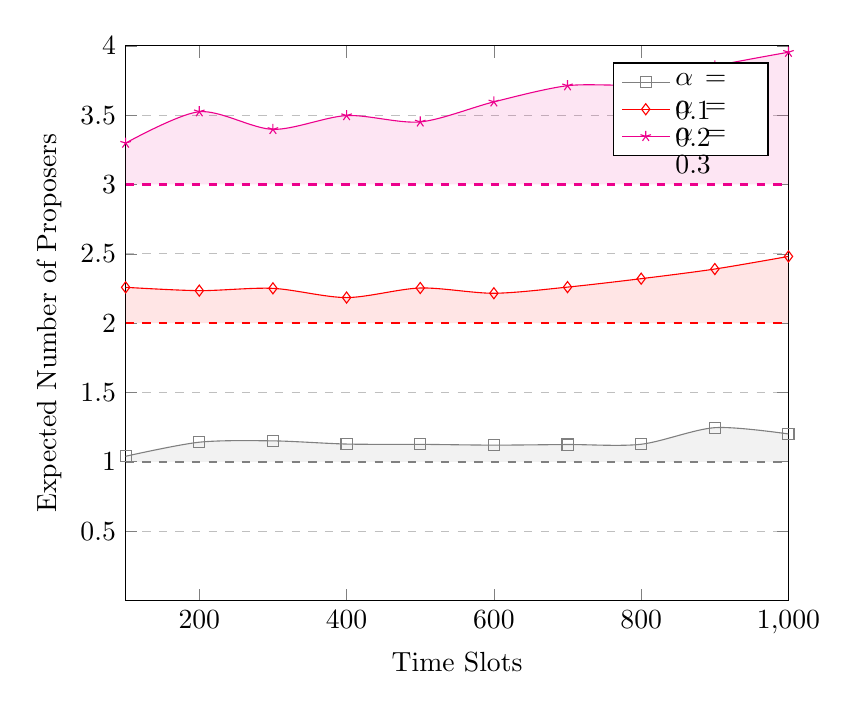
\begin{tikzpicture}
\begin{axis}[
    title={},
    xlabel={Time Slots}, % ($\times 100$},
    ylabel={Expected Number of Proposers},
    xmin=100, xmax=1000,
    ymin=0.0, ymax=4.0,
    xtick={200,400,600,800,1000},
    ytick={0.5,1.0,1.5,2.0,2.5,3.0, 3.5,4.0},
    legend pos=north east,
    ymajorgrids=true,
    grid style=dashed,
]

\addplot[
	smooth,
    name path=f01,
    color=gray,
    mark=square,
    ]
    coordinates {
(100.0 ,1.0396)
(200.0 ,1.1410)
 (300.0 ,1.1507)
(400.0 ,1.1277)
 (500.0 ,1.1256)
(600.0 ,1.1200)
 (700.0 ,1.1243)
 (800.0 ,1.1263)
 (900.0 ,1.2459)
(1000.0 ,1.2005)
    };
    \addlegendentry[text width=1cm]{$\alpha = 0.1$}

\draw[gray,dashed,thick] (axis cs:100, 0.9999) -- (axis cs:1000, 0.9999);
\path[name path=b01] (axis cs:100, 0.9999) -- (axis cs:1000, 0.9999);

    \addplot [
        thick,
        color=gray,
        fill=gray, 
        fill opacity=0.1,
        forget plot
    ]
    fill between[
        of=f01 and b01,
        soft clip second={domain=100:1000}
    ];
    
\addplot[
	smooth,
    name path=f02,
    color=red,
    mark=diamond,
    ]
    coordinates {
(100.0 ,2.2582)
(200.0 ,2.2341)
 (300.0 ,2.2507)
(400.0 ,2.1842)
 (500.0 ,2.2532)
(600.0 ,2.2153)
 (700.0 ,2.2597)
 (800.0 ,2.3205)
 (900.0 ,2.3901)
(1000.0 ,2.4810)
    };
    \addlegendentry[text width=1cm]{$\alpha = 0.2$}

\draw[red,dashed,thick] (axis cs:100, 1.9999) -- (axis cs:1000, 1.9999);
\path[name path=b02] (axis cs:100, 1.9999) -- (axis cs:1000, 1.9999);

    \addplot [
        thick,
        color=red,
        fill=red, 
        fill opacity=0.1,
        forget plot
    ]
    fill between[
        of=f02 and b02,
        soft clip second={domain=100:1000}
    ];
    
\addplot[
	smooth,
    name path=f03,
    color=magenta,
    mark=star,
    ]
    coordinates {
(100.0 ,3.2983)
(200.0 ,3.5247)
 (300.0 ,3.3974)
(400.0 ,3.4969)
 (500.0 ,3.4512)
(600.0 ,3.5958)
 (700.0 ,3.7123)
 (800.0 ,3.7244)
 (900.0 ,3.8542)
(1000.0 ,3.9538)
    };
    \addlegendentry[text width=1cm]{$\alpha = 0.3$}

\draw[magenta,dashed,thick] (axis cs:100, 2.9999) -- (axis cs:1000, 2.9999);
\path[name path=b03] (axis cs:100, 2.9999) -- (axis cs:1000, 2.9999);

    \addplot [
        thick,
        color=magenta,
        fill=magenta, 
        fill opacity=0.1,
        forget plot
    ]
    fill between[
        of=f03 and b03,
        soft clip second={domain=100:1000}
    ];
%\addplot[
%	smooth,
%    color=blue,
%    mark=+,
%    ]
%    coordinates {
%(10.0 ,0)
%(50.0 ,0)
%(100.0 ,0)
%(500.0 ,0)
%(1000.0 ,0)
%    };
%    \addlegendentry[text width=1cm]{$\alpha = 0.4$}
%
%\addplot[
%	smooth, tension=0.2,
%    color=brown,
%    mark=pentagon,
%    ]
%    coordinates {
%(10.0 ,0)
%(50.0 ,0)
%(100.0 ,0)
%(500.0 ,0)
%(1000.0 ,0)
%    };
%    \addlegendentry[text width=1cm]{$\alpha = 0.5$}

%\addplot[
%	smooth, tension=0.2,
%    color=cyan,
%    mark=*,
%    ]
%    coordinates {
%(1 ,0.0000)
%(5 ,0.7879)
%(10 ,0.8540)
%(15 ,0.8807)
%(20 ,0.9077)
%(25 ,0.9253)
%(30 ,0.9356)
%(35 ,0.9497)
%(40 ,0.9619)
%(45 ,0.9648)
%(50 ,1.0000)
%    };
%    \addlegendentry[text width=1cm]{AG}


\end{axis}
\end{tikzpicture}
}
		\label{chr:ms_sf0_10x500}} \\
	\subfloat[][MS (SF0, 10x1000)]{
		\resizebox{0.4\textwidth}{!}{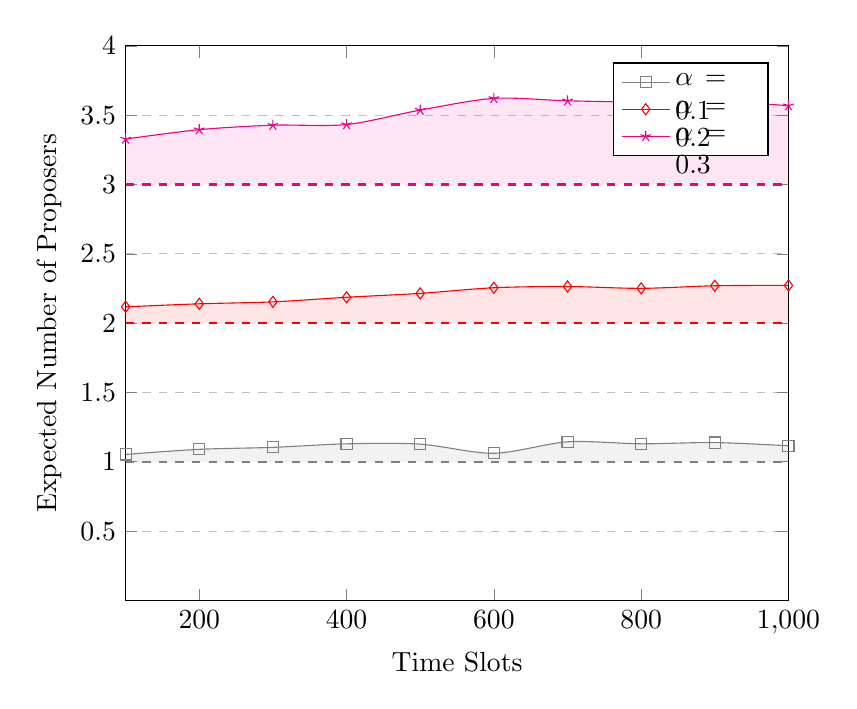
\begin{tikzpicture}
\begin{axis}[
    title={},
    xlabel={Time Slots}, % ($\times 100$},
    ylabel={Expected Number of Proposers},
    xmin=100, xmax=1000,
    ymin=0.0, ymax=4.0,
    xtick={200,400,600,800,1000},
    ytick={0.5,1.0,1.5,2.0,2.5,3.0, 3.5,4.0},
    legend pos=north east,
    ymajorgrids=true,
    grid style=dashed,
]

\addplot[
	smooth,
    name path=f01,
    color=gray,
    mark=square,
    ]
    coordinates {
(100.0 ,1.0529)
(200.0 ,1.0896)
 (300.0 ,1.1039)
(400.0 ,1.1293)
 (500.0 ,1.127)
(600.0 ,1.0610)
 (700.0 ,1.1439)
 (800.0 ,1.1295)
 (900.0 ,1.1384)
(1000.0 ,1.1151)
    };
    \addlegendentry[text width=1cm]{$\alpha = 0.1$}

\draw[gray,dashed,thick] (axis cs:100, 0.9999) -- (axis cs:1000, 0.9999);
\path[name path=b01] (axis cs:100, 0.9999) -- (axis cs:1000, 0.9999);

    \addplot [
        thick,
        color=gray,
        fill=gray, 
        fill opacity=0.1,
        forget plot
    ]
    fill between[
        of=f01 and b01,
        soft clip second={domain=100:1000}
    ];
    
\addplot[
	smooth,
    name path=f02,
    color=red,
    mark=diamond,
    ]
    coordinates {
(100.0 ,2.1176)
(200.0 ,2.1392)
 (300.0 ,2.1532)
(400.0 ,2.1864)
 (500.0 ,2.2145)
(600.0 ,2.2551)
 (700.0 ,2.2639)
 (800.0 ,2.2508)
 (900.0 ,2.2694)
(1000.0 ,2.2722)
    };
    \addlegendentry[text width=1cm]{$\alpha = 0.2$}

\draw[red,dashed,thick] (axis cs:100, 1.9999) -- (axis cs:1000, 1.9999);
\path[name path=b02] (axis cs:100, 1.9999) -- (axis cs:1000, 1.9999);

    \addplot [
        thick,
        color=red,
        fill=red, 
        fill opacity=0.1,
        forget plot
    ]
    fill between[
        of=f02 and b02,
        soft clip second={domain=100:1000}
    ];
    
\addplot[
	smooth,
     name path=f03,
   color=magenta,
    mark=star,
    ]
    coordinates {
(100.0 ,3.3277)
(200.0 ,3.3952)
 (300.0 ,3.4276)
(400.0 ,3.4322)
 (500.0 ,3.5363)
(600.0 ,3.6210)
 (700.0 ,3.6034)
 (800.0 ,3.5948)
 (900.0 ,3.6012)
(1000.0 ,3.5681)
    };
    \addlegendentry[text width=1cm]{$\alpha = 0.3$}

\draw[magenta,dashed,thick] (axis cs:100, 2.9999) -- (axis cs:1000, 2.9999);
\path[name path=b03] (axis cs:100, 2.9999) -- (axis cs:1000, 2.9999);

    \addplot [
        thick,
        color=magenta,
        fill=magenta, 
        fill opacity=0.1,
        forget plot
    ]
    fill between[
        of=f03 and b03,
        soft clip second={domain=100:1000}
    ];
    
%\addplot[
%	smooth,
%    color=blue,
%    mark=+,
%    ]
%    coordinates {
%(10.0 ,0)
%(50.0 ,0)
%(100.0 ,0)
%(500.0 ,0)
%(1000.0 ,0)
%    };
%    \addlegendentry[text width=1cm]{$\alpha = 0.4$}
%
%\addplot[
%	smooth, tension=0.2,
%    color=brown,
%    mark=pentagon,
%    ]
%    coordinates {
%(10.0 ,0)
%(50.0 ,0)
%(100.0 ,0)
%(500.0 ,0)
%(1000.0 ,0)
%    };
%    \addlegendentry[text width=1cm]{$\alpha = 0.5$}

%\addplot[
%	smooth, tension=0.2,
%    color=cyan,
%    mark=*,
%    ]
%    coordinates {
%(1 ,0.0000)
%(5 ,0.7879)
%(10 ,0.8540)
%(15 ,0.8807)
%(20 ,0.9077)
%(25 ,0.9253)
%(30 ,0.9356)
%(35 ,0.9497)
%(40 ,0.9619)
%(45 ,0.9648)
%(50 ,1.0000)
%    };
%    \addlegendentry[text width=1cm]{AG}


\end{axis}
\end{tikzpicture}
}
		\label{chr:ms_sf0_10x1000}}
	\caption{The expected number of attacker-controlled proposers in the proposers list against execution time in time slots, assuming the attacker is attempting to maximize the number of compromised proposers (\texttt{\#SCORE-FUNCTION} is $0$). The dashed lines represent the base values (with no active attack) computed using Equation~(\ref{eqn:ex_ms}). The shaded areas visualize the expected bias achievable by the attacker for the three different attack probabilities plotted. We assume a proposers list of size $10$, and a validator set of size (a) $10\times 500$ and (b) $10\times 1000$.}
	\label{chr:ms_sf0}
\end{figure}
%
\begin{figure}%[t!]
	\captionsetup{farskip=0pt}% <--- no gap at the top
	\centering
%	\subfloat[][10x100]{
%		\resizebox{0.4\textwidth}{!}{\input{charts/ms_sf1_10x100}}
%		\label{chr:ms_sf1_10x100}} \\
	\subfloat[][MS (SF1, 10x500)]{
		\resizebox{0.4\textwidth}{!}{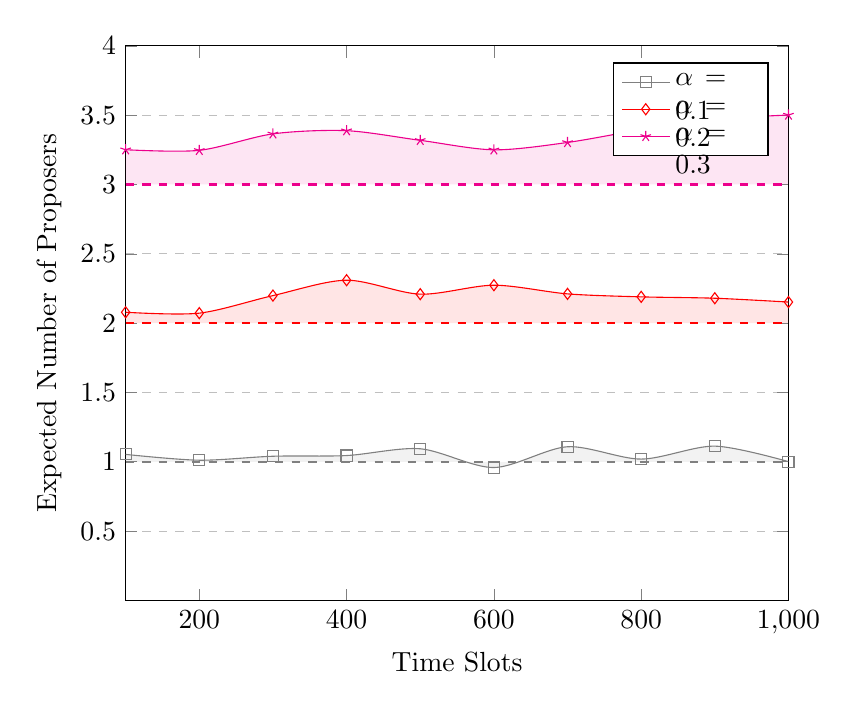
\begin{tikzpicture}
\begin{axis}[
    title={},
    xlabel={Time Slots}, % ($\times 100$},
    ylabel={Expected Number of Proposers},
    xmin=100, xmax=1000,
    ymin=0.0, ymax=4.0,
    xtick={200,400,600,800,1000},
    ytick={0.5,1.0,1.5,2.0,2.5,3.0, 3.5,4.0},
    legend pos=north east,
    ymajorgrids=true,
    grid style=dashed,
]

\addplot[
	smooth,
    name path=f01,
    color=gray,
    mark=square,
    ]
    coordinates {
(100.0 ,1.0531)
(200.0 ,1.0112)
 (300.0 ,1.0398)
(400.0 ,1.0448)
 (500.0 ,1.0937)
(600.0 ,0.9583)
 (700.0 ,1.1084)
 (800.0 ,1.0193)
 (900.0 ,1.1128)
(1000.0 ,1.0009)
    };
    \addlegendentry[text width=1cm]{$\alpha = 0.1$}
\draw[gray,dashed,thick] (axis cs:100, 0.9999) -- (axis cs:1000, 0.9999);
\path[name path=b01] (axis cs:100, 0.9999) -- (axis cs:1000, 0.9999);

    \addplot [
        thick,
        color=gray,
        fill=gray, 
        fill opacity=0.1,
        forget plot
    ]
    fill between[
        of=f01 and b01,
        soft clip second={domain=100:1000}
    ];
    
    
\addplot[
	smooth,
    name path=f02,
    color=red,
    mark=diamond,
    ]
    coordinates {
(100.0 ,2.0783)
(200.0 ,2.0718)
 (300.0 ,2.1984)
(400.0 ,2.3095)
 (500.0 ,2.2087)
(600.0 ,2.2734)
 (700.0 ,2.2108)
 (800.0 ,2.1893)
 (900.0 ,2.1794)
(1000.0 ,2.1518)
    };
    \addlegendentry[text width=1cm]{$\alpha = 0.2$}
\draw[red,dashed,thick] (axis cs:100, 1.9999) -- (axis cs:1000, 1.9999);
\path[name path=b02] (axis cs:100, 1.9999) -- (axis cs:1000, 1.9999);

    \addplot [
        thick,
        color=red,
        fill=red, 
        fill opacity=0.1,
        forget plot
    ]
    fill between[
        of=f02 and b02,
        soft clip second={domain=100:1000}
    ];
    
    
\addplot[
	smooth,
    name path=f03,
    color=magenta,
    mark=star,
    ]
    coordinates {
(100.0 ,3.2505)
(200.0 ,3.2461)
 (300.0 ,3.3649)
(400.0 ,3.3879)
 (500.0 ,3.3183)
(600.0 ,3.2498)
 (700.0 ,3.3029)
 (800.0 ,3.3947)
 (900.0 ,3.4698)
(1000.0 ,3.5008)
    };
    \addlegendentry[text width=1cm]{$\alpha = 0.3$}
\draw[magenta,dashed,thick] (axis cs:100, 2.9999) -- (axis cs:1000, 2.9999);
\path[name path=b03] (axis cs:100, 2.9999) -- (axis cs:1000, 2.9999);

    \addplot [
        thick,
        color=magenta,
        fill=magenta, 
        fill opacity=0.1,
        forget plot
    ]
    fill between[
        of=f03 and b03,
        soft clip second={domain=100:1000}
    ];
%\addplot[
%	smooth,
%    color=blue,
%    mark=+,
%    ]
%    coordinates {
%(10.0 ,0)
%(50.0 ,0)
%(100.0 ,0)
%(500.0 ,0)
%(1000.0 ,0)
%    };
%    \addlegendentry[text width=1cm]{$\alpha = 0.4$}
%
%\addplot[
%	smooth, tension=0.2,
%    color=brown,
%    mark=pentagon,
%    ]
%    coordinates {
%(10.0 ,0)
%(50.0 ,0)
%(100.0 ,0)
%(500.0 ,0)
%(1000.0 ,0)
%    };
%    \addlegendentry[text width=1cm]{$\alpha = 0.5$}

%\addplot[
%	smooth, tension=0.2,
%    color=cyan,
%    mark=*,
%    ]
%    coordinates {
%(1 ,0.0000)
%(5 ,0.7879)
%(10 ,0.8540)
%(15 ,0.8807)
%(20 ,0.9077)
%(25 ,0.9253)
%(30 ,0.9356)
%(35 ,0.9497)
%(40 ,0.9619)
%(45 ,0.9648)
%(50 ,1.0000)
%    };
%    \addlegendentry[text width=1cm]{AG}


\end{axis}
\end{tikzpicture}
}
		\label{chr:ms_sf1_10x500}} \\
	\subfloat[][MS (SF1, 10x1000)]{
		\resizebox{0.4\textwidth}{!}{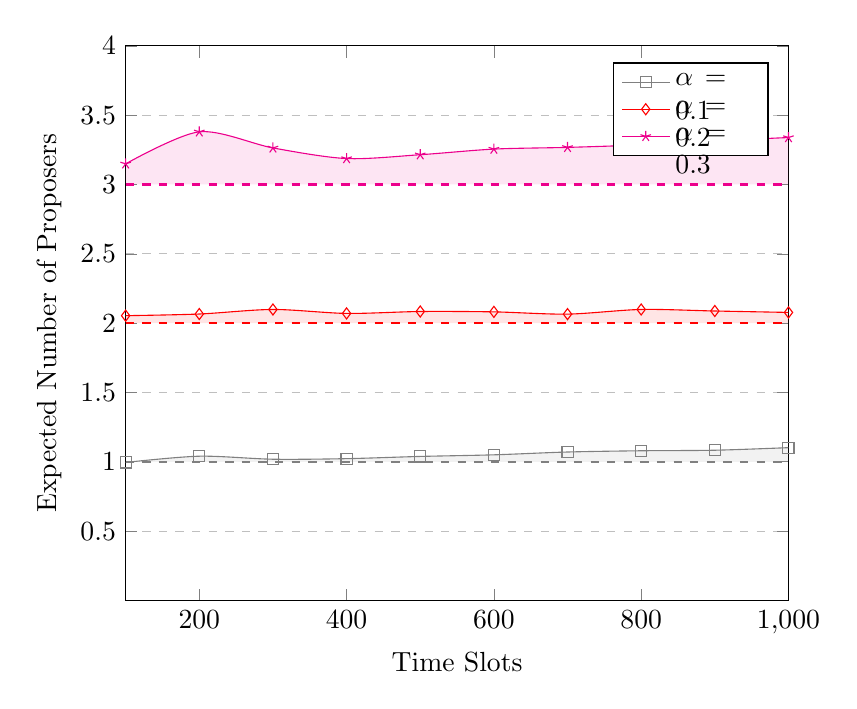
\begin{tikzpicture}
\begin{axis}[
    title={},
    xlabel={Time Slots}, % ($\times 100$},
    ylabel={Expected Number of Proposers},
    xmin=100, xmax=1000,
    ymin=0.0, ymax=4.0,
    xtick={200,400,600,800,1000},
    ytick={0.5,1.0,1.5,2.0,2.5,3.0, 3.5,4.0},
    legend pos=north east,
    ymajorgrids=true,
    grid style=dashed,
]

\addplot[
	smooth,
    name path=f01,
    color=gray,
    mark=square,
    ]
    coordinates {
(100.0 ,0.9952)
(200.0 ,1.0401)
 (300.0 ,1.0183)
(400.0 ,1.0224)
 (500.0 ,1.0384)
(600.0 ,1.0500)
 (700.0 ,1.0703)
 (800.0 ,1.0793)
 (900.0 ,1.0832)
(1000.0 ,1.1017)
    };
    \addlegendentry[text width=1cm]{$\alpha = 0.1$}
\draw[gray,dashed,thick] (axis cs:100, 0.9999) -- (axis cs:1000, 0.9999);
\path[name path=b01] (axis cs:100, 0.9999) -- (axis cs:1000, 0.9999);

    \addplot [
        thick,
        color=gray,
        fill=gray, 
        fill opacity=0.1,
        forget plot
    ]
    fill between[
        of=f01 and b01,
        soft clip second={domain=100:1000}
    ];
    
\addplot[
	smooth,
    name path=f02,
    color=red,
    mark=diamond,
    ]
    coordinates {
(100.0 ,2.0536)
(200.0 ,2.0656)
 (300.0 ,2.0984)
(400.0 ,2.0699)
 (500.0 ,2.0837)
(600.0 ,2.0811)
 (700.0 ,2.0649)
 (800.0 ,2.0984)
 (900.0 ,2.0873)
(1000.0 ,2.0771)
    };
    \addlegendentry[text width=1cm]{$\alpha = 0.2$}
\draw[red,dashed,thick] (axis cs:100, 1.9999) -- (axis cs:1000, 1.9999);
\path[name path=b02] (axis cs:100, 1.9999) -- (axis cs:1000, 1.9999);

    \addplot [
        thick,
        color=red,
        fill=red, 
        fill opacity=0.1,
        forget plot
    ]
    fill between[
        of=f02 and b02,
        soft clip second={domain=100:1000}
    ];
    
\addplot[
	smooth,
    name path=f03,
    color=magenta,
    mark=star,
    ]
    coordinates {
(100.0 ,3.1486)
(200.0 ,3.3796)
 (300.0 ,3.2635)
(400.0 ,3.1869)
 (500.0 ,3.2145)
(600.0 ,3.2551)
 (700.0 ,3.2674)
 (800.0 ,3.2853)
 (900.0 ,3.3144)
(1000.0 ,3.3384)
    };
    \addlegendentry[text width=1cm]{$\alpha = 0.3$}
\draw[magenta,dashed,thick] (axis cs:100, 2.9999) -- (axis cs:1000, 2.9999);
\path[name path=b03] (axis cs:100, 2.9999) -- (axis cs:1000, 2.9999);

    \addplot [
        thick,
        color=magenta,
        fill=magenta, 
        fill opacity=0.1,
        forget plot
    ]
    fill between[
        of=f03 and b03,
        soft clip second={domain=100:1000}
    ];
%\addplot[
%	smooth,
%    color=blue,
%    mark=+,
%    ]
%    coordinates {
%(10.0 ,0)
%(50.0 ,0)
%(100.0 ,0)
%(500.0 ,0)
%(1000.0 ,0)
%    };
%    \addlegendentry[text width=1cm]{$\alpha = 0.4$}
%
%\addplot[
%	smooth, tension=0.2,
%    color=brown,
%    mark=pentagon,
%    ]
%    coordinates {
%(10.0 ,0)
%(50.0 ,0)
%(100.0 ,0)
%(500.0 ,0)
%(1000.0 ,0)
%    };
%    \addlegendentry[text width=1cm]{$\alpha = 0.5$}

%\addplot[
%	smooth, tension=0.2,
%    color=cyan,
%    mark=*,
%    ]
%    coordinates {
%(1 ,0.0000)
%(5 ,0.7879)
%(10 ,0.8540)
%(15 ,0.8807)
%(20 ,0.9077)
%(25 ,0.9253)
%(30 ,0.9356)
%(35 ,0.9497)
%(40 ,0.9619)
%(45 ,0.9648)
%(50 ,1.0000)
%    };
%    \addlegendentry[text width=1cm]{AG}


\end{axis}
\end{tikzpicture}
}
		\label{chr:ms_sf1_10x1000}}
	\caption{The expected number of attacker-controlled proposers in the proposers list against execution time in time slots, assuming the attacker is attempting to maximize the length of the compromised tail (\texttt{\#SCORE-FUNCTION} is $1$). The dashed lines represent the base values (with no active attack) computed using Equation~(\ref{eqn:ex_ms}). The shaded areas visualize the expected bias achievable by the attacker for the three different attack probabilities plotted. We assume a proposers list of size $10$, and a validator set of size (a) $10\times 500$ and (b) $10\times 1000$.}
	\label{chr:ms_sf1}
\end{figure}



\subsection{Last-Word Score (LWS)}
\label{sec:lws}

As for MS, we compute a baseline value for LWS. This value represents the expected length of the longest attacker-controlled tail of the proposers list in a round of the RANDAO process \textit{assuming the attacker is not pre-computing reveal strategies}. This value is computed as follows.

Let $a$ be the event of picking an attacker-controlled validator, which has probability $p$, and $b$ the event of picking an honest validator $b$, having probability $(1-p)$. Let the cycle length (length of the proposers list) be $k$. A compromised tail in the proposers list corresponds to either a sequence of events $a$ of length $j < k$ followed immediately by exactly one occurrence of event $b$, or a sequence of events $a$ of length exactly $k$ (the whole list is controlled by the attacker). Therefore, letting $X$ be a random variable corresponding to the length of the longest compromised tail, we have:
\[
Pr[X = i] = 
	\begin{cases}
	p^i (1-p)		&  i < k \\
	p^i				&  i = k
	\end{cases}
\]
Therefore, the expected value of $X$ is
\begin{equation}\label{eqn:ex_lws}
EX[X] = \sum_{i=0}^{k-1} i \cdot p^i (1-p) + k \cdot p^k
\end{equation}
(Note that the distribution of $X$ is \textit{almost} geometric with success probability $1-p$). For example, assuming $p = 0.2$, the expected number of proposers in the longest attacker-controlled tail of a list of length $k = 10$ is approximately $0.25$ (assuming the attacker is following the protocol).    

However, when the attacker pre-computes strategies, the expectation will likely be different. As for the MS property above, to evaluate this potential bias, we similarly specify the property LWS using the following formula:
\begin{equation}
\begin{split}
\mathit{lws}(t) = \; 
	& \mathbf{\underline{if}} \; \mathit{time}() > t \; \mathbf{\underline{then}} \; \mathit{countCompromisedTail}() \\ 
	& \mathbf{\underline{else}} \; \bigcirc \mathit{lws}(t) \;\mathbf{\underline{fi}} \; ; \\
                       & \mathbf{\underline{eval}}\; \mathbf{E}[\mathit{lws}(t_0)] 
\end{split}
\end{equation}
The formula has a similar structure to that of the MS property in (\ref{eqn:ms_quatex}), except that the state function $\mathit{countCompromisedTail}()$ is used, which counts the number of proposers in the longest compromised tail in the proposers list of the current state of the RANDAO object. As before, estimating the expectation expression $\mathbf{E}[\mathit{lws}(t_0)]$ gives an approximation of the expected length of the longest compromised tail that an attacker can achieve within the specified time limit. We use our model to statistically model check this formula using the same verification parameters used for the property MS above (a $95\%$ confidence interval with size at most $0.02$ and a perfectly reliable communication network).

In our analysis of the LWS property, we consider (again) the two possible attack strategies: (1) maximizing the number of compromised proposers (\verb+countCompromised+) and (2) maximizing the length of the compromised tail (\verb+countCompromisedTail+). The results of the former are plotted in the charts of Figure~\ref{chr:lws_sf0}, while the analysis results of the latter are shown in Figure~\ref{chr:lws_sf1}.

The charts in Figure~\ref{chr:lws_sf0} make it clear that this strategy is only somewhat effective in mounting an attack. The gains are small at all attack levels, and do not seem to grow as the number of rounds increases. For example, a $0.2$ attacker is only able to achieve a compromised tail of length around $0.4$ (on average), which is only $0.15$ proposers beyond the baseline $0.25$, even at large numbers of rounds. The gains are higher though for larger attack probabilities, but only marginally.

The second strategy is only slightly better. As Figure~\ref{chr:lws_sf1} shows, maximizing the length of the compromised tail can result in a steady and reliable effect on the proposers list. As the attack probability increases, the bias achieved can  be greater within shorter periods of time. For example, at around 60 rounds, the bias achieved by a $0.1$ attacker is negligible, while a $0.2$ attacker is expected to achieve 20\% gains over the baseline (at around $0.32$ compared with $0.25$), and a $0.3$ attacker achieves 60\% gains (at around $0.7$ compared with $0.43$). Nevertheless, even at high attack rates, the charts do not show strong increasing trends, suggesting that any gains more significant than those would require applying reveal strategies for very extended periods of time. %At around 100 rounds, the $0.2$ attacker is already expected to attain a compromised tail of length $2$, which represents a significant bias level. Higher attack levels can potentially result in compromising the entire proposers list, enabling the attacker to gain control of the system.

%
\begin{figure}%[t!]
	\captionsetup{farskip=0pt}% <--- no gap at the top
	\centering
%	\subfloat[][10x100]{
%		\resizebox{0.4\textwidth}{!}{\input{charts/lws_sf0_10x100}}
%		\label{chr:lws_sf0_10x100}} \\
	\subfloat[][LWS (SF0, 10x500)]{
		\resizebox{0.4\textwidth}{!}{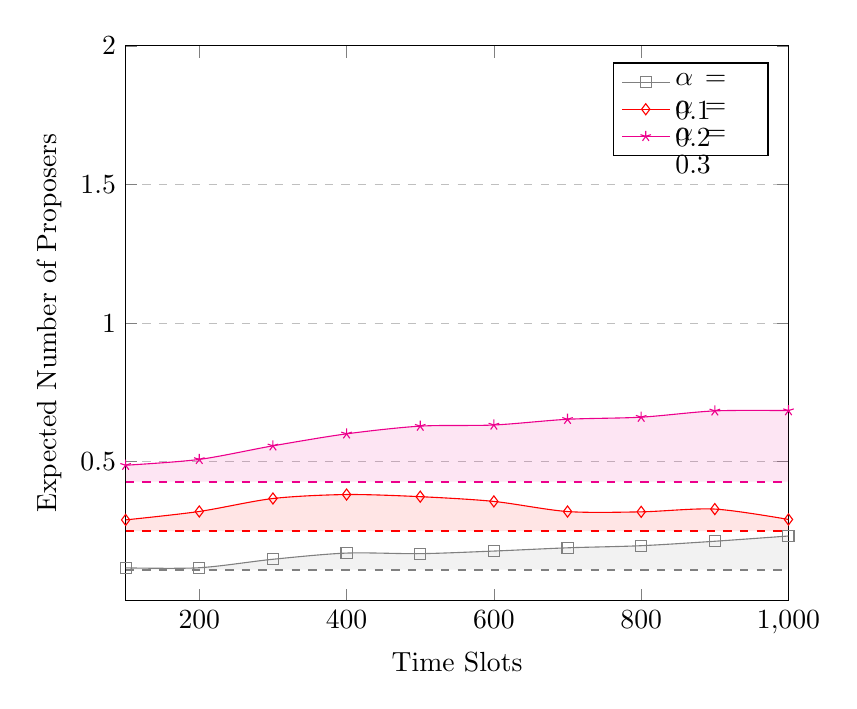
\begin{tikzpicture}
\begin{axis}[
    title={},
    xlabel={Time Slots}, % ($\times 100$},
    ylabel={Expected Number of Proposers},
    xmin=100, xmax=1000,
    ymin=0.0, ymax=2.0,
    xtick={200,400,600,800,1000},
    ytick={0.5,1.0,1.5,2.0},
    legend pos=north east,
    ymajorgrids=true,
    grid style=dashed,
]

\addplot[
	smooth,
     name path=f01,
    color=gray,
    mark=square,
    ]
    coordinates {
(100.0 ,0.1174)
(200.0 ,0.1178)
 (300.0 ,0.1484)
(400.0 ,0.1707)
 (500.0 ,0.1686)
(600.0 ,0.1780)
 (700.0 ,0.1897)
 (800.0 ,0.1973)
 (900.0 ,0.2134)
(1000.0 ,0.2323)
    };
    \addlegendentry[text width=1cm]{$\alpha = 0.1$}
\draw[gray,dashed,thick] (axis cs:100, 0.1111) -- (axis cs:1000, 0.1111);
\path[name path=b01] (axis cs:100, 0.1111) -- (axis cs:1000, 0.1111);

    \addplot [
        thick,
        color=gray,
        fill=gray, 
        fill opacity=0.1,
        forget plot
    ]
    fill between[
        of=f01 and b01,
        soft clip second={domain=100:1000}
    ];
    
    
\addplot[
	smooth,
    name path=f02,
    color=red,
    mark=diamond,
    ]
    coordinates {
(100.0 ,0.2904)
(200.0 ,0.3208)
 (300.0 ,0.3675)
(400.0 ,0.3818)
 (500.0 ,0.3741)
(600.0 ,0.3570)
 (700.0 ,0.3205)
 (800.0 ,0.3194)
 (900.0 ,0.3294)
(1000.0 ,0.2920)
    };
    \addlegendentry[text width=1cm]{$\alpha = 0.2$}
\draw[red,dashed,thick] (axis cs:100, 0.2499) -- (axis cs:1000, 0.2499);
\path[name path=b02] (axis cs:100, 0.2499) -- (axis cs:1000, 0.2499);

    \addplot [
        thick,
        color=red,
        fill=red, 
        fill opacity=0.1,
        forget plot
    ]
    fill between[
        of=f02 and b02,
        soft clip second={domain=100:1000}
    ];
    
    
\addplot[
	smooth,
    name path=f03,
    color=magenta,
    mark=star,
    ]
    coordinates {
(100.0 ,0.4875)
(200.0 ,0.5085)		%
 (300.0 ,0.5575)	%
(400.0 ,0.6007)		%
 (500.0 ,0.6285)	
(600.0 ,0.6326)		%	
 (700.0 ,0.6532)	%
 (800.0 ,0.6608)	%	
 (900.0 ,0.6835)	%
(1000.0 ,0.6845)	%
    };
    \addlegendentry[text width=1cm]{$\alpha = 0.3$}
\draw[magenta,dashed,thick] (axis cs:100, 0.4284) -- (axis cs:1000, 0.4284);
\path[name path=b03] (axis cs:100, 0.4284) -- (axis cs:1000, 0.4284);

    \addplot [
        thick,
        color=magenta,
        fill=magenta, 
        fill opacity=0.1,
        forget plot
    ]
    fill between[
        of=f03 and b03,
        soft clip second={domain=100:1000}
    ];
    
    
%\addplot[
%	smooth,
%    color=blue,
%    mark=+,
%    ]
%    coordinates {
%(10.0 ,0)
%(50.0 ,0)
%(100.0 ,0)
%(500.0 ,0)
%(1000.0 ,0)
%    };
%    \addlegendentry[text width=1cm]{$\alpha = 0.4$}
%
%\addplot[
%	smooth, tension=0.2,
%    color=brown,
%    mark=pentagon,
%    ]
%    coordinates {
%(10.0 ,0)
%(50.0 ,0)
%(100.0 ,0)
%(500.0 ,0)
%(1000.0 ,0)
%    };
%    \addlegendentry[text width=1cm]{$\alpha = 0.5$}

%\addplot[
%	smooth, tension=0.2,
%    color=cyan,
%    mark=*,
%    ]
%    coordinates {
%(1 ,0.0000)
%(5 ,0.7879)
%(10 ,0.8540)
%(15 ,0.8807)
%(20 ,0.9077)
%(25 ,0.9253)
%(30 ,0.9356)
%(35 ,0.9497)
%(40 ,0.9619)
%(45 ,0.9648)
%(50 ,1.0000)
%    };
%    \addlegendentry[text width=1cm]{AG}


\end{axis}
\end{tikzpicture}
}
		\label{chr:lws_sf0_10x500}} \\
	\subfloat[][LWS (SF0, 10x1000)]{
		\resizebox{0.4\textwidth}{!}{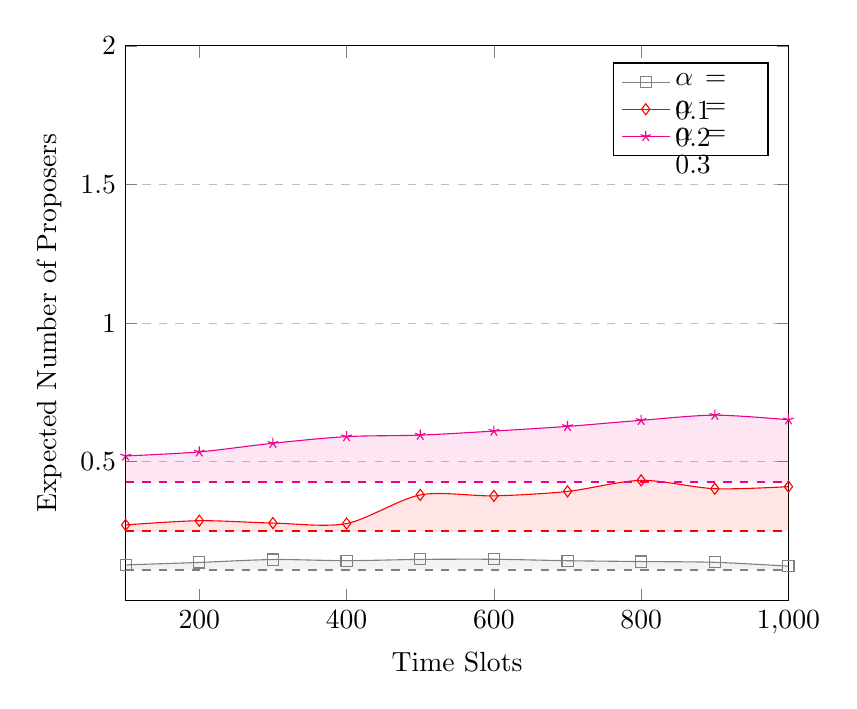
\begin{tikzpicture}
\begin{axis}[
    title={},
    xlabel={Time Slots}, % ($\times 100$},
    ylabel={Expected Number of Proposers},
    xmin=100, xmax=1000,
    ymin=0.0, ymax=2.0,
    xtick={200,400,600,800,1000},
    ytick={0.5,1.0,1.5,2.0},
    legend pos=north east,
    ymajorgrids=true,
    grid style=dashed,
]

\addplot[
	smooth,
    name path=f01,
    color=gray,
    mark=square,
    ]
    coordinates {
(100.0 ,0.1281)
(200.0 ,0.1370)
 (300.0 ,0.1474)
(400.0 ,0.1433)
 (500.0 ,0.1479)
(600.0 ,0.1484)
 (700.0 ,0.1432)
 (800.0 ,0.1402)
 (900.0 ,0.1374)
(1000.0 ,0.1236)
    };
    \addlegendentry[text width=1cm]{$\alpha = 0.1$}
\draw[gray,dashed,thick] (axis cs:100, 0.1111) -- (axis cs:1000, 0.1111);
\path[name path=b01] (axis cs:100, 0.1111) -- (axis cs:1000, 0.1111);

    \addplot [
        thick,
        color=gray,
        fill=gray, 
        fill opacity=0.1,
        forget plot
    ]
    fill between[
        of=f01 and b01,
        soft clip second={domain=100:1000}
    ];
    
    
\addplot[
	smooth,
    name path=f02,
    color=red,
    mark=diamond,
    ]
    coordinates {
(100.0 ,0.2722)
(200.0 ,0.2875)
 (300.0 ,0.2790)
(400.0 ,0.2772)
 (500.0 ,0.3805)
(600.0 ,0.3770)
 (700.0 ,0.3931)
 (800.0 ,0.4329)
 (900.0 ,0.4028)
(1000.0 ,0.4103)
    };
    \addlegendentry[text width=1cm]{$\alpha = 0.2$}
\draw[red,dashed,thick] (axis cs:100, 0.2499) -- (axis cs:1000, 0.2499);
\path[name path=b02] (axis cs:100, 0.2499) -- (axis cs:1000, 0.2499);

    \addplot [
        thick,
        color=red,
        fill=red, 
        fill opacity=0.1,
        forget plot
    ]
    fill between[
        of=f02 and b02,
        soft clip second={domain=100:1000}
    ];
    
\addplot[
	smooth,
    name path=f03,
    color=magenta,
    mark=star,
    ]
    coordinates {
(100.0 ,0.5210)		
(200.0 ,0.5356)		%
 (300.0 ,0.5668)	%
(400.0 ,0.5907)		%
 (500.0 ,0.5961)	
(600.0 ,0.6107)		%
 (700.0 ,0.6276)	%
 (800.0 ,0.6495)	%
 (900.0 ,0.6681)	%
(1000.0 ,0.6515)	%
    };
    \addlegendentry[text width=1cm]{$\alpha = 0.3$}
\draw[magenta,dashed,thick] (axis cs:100, 0.4284) -- (axis cs:1000, 0.4284);
\path[name path=b03] (axis cs:100, 0.4284) -- (axis cs:1000, 0.4284);

    \addplot [
        thick,
        color=magenta,
        fill=magenta, 
        fill opacity=0.1,
        forget plot
    ]
    fill between[
        of=f03 and b03,
        soft clip second={domain=100:1000}
    ];
    
    
%\addplot[
%	smooth,
%    color=blue,
%    mark=+,
%    ]
%    coordinates {
%(10.0 ,0)
%(50.0 ,0)
%(100.0 ,0)
%(500.0 ,0)
%(1000.0 ,0)
%    };
%    \addlegendentry[text width=1cm]{$\alpha = 0.4$}
%
%\addplot[
%	smooth, tension=0.2,
%    color=brown,
%    mark=pentagon,
%    ]
%    coordinates {
%(10.0 ,0)
%(50.0 ,0)
%(100.0 ,0)
%(500.0 ,0)
%(1000.0 ,0)
%    };
%    \addlegendentry[text width=1cm]{$\alpha = 0.5$}

%\addplot[
%	smooth, tension=0.2,
%    color=cyan,
%    mark=*,
%    ]
%    coordinates {
%(1 ,0.0000)
%(5 ,0.7879)
%(10 ,0.8540)
%(15 ,0.8807)
%(20 ,0.9077)
%(25 ,0.9253)
%(30 ,0.9356)
%(35 ,0.9497)
%(40 ,0.9619)
%(45 ,0.9648)
%(50 ,1.0000)
%    };
%    \addlegendentry[text width=1cm]{AG}


\end{axis}
\end{tikzpicture}
}
		\label{chr:lws_sf0_10x1000}}
	\caption{The expected number of attacker-controlled proposers in the proposers list against execution time in time slots, assuming the attacker is attempting to maximize the number of compromised proposers (\texttt{\#SCORE-FUNCTION} is $0$). The dashed lines represent the base values (with no active attack) computed using Equation~(\ref{eqn:ex_lws}). The shaded areas visualize the expected bias achievable by the attacker for the three different attack probabilities plotted. We assume a proposers list of size $10$, and a validator set of size (a) $10\times 500$ and (b) $10\times 1000$.}
	\label{chr:lws_sf0}
\end{figure}
%
\begin{figure}%[t!]
	\captionsetup{farskip=0pt}% <--- no gap at the top
	\centering
%	\subfloat[][10x100]{
%		\resizebox{0.4\textwidth}{!}{\input{charts/lws_sf1_10x100}}
%		\label{chr:lws_sf1_10x100}} \\
	\subfloat[][LWS (SF1, 10x500)]{
		\resizebox{0.4\textwidth}{!}{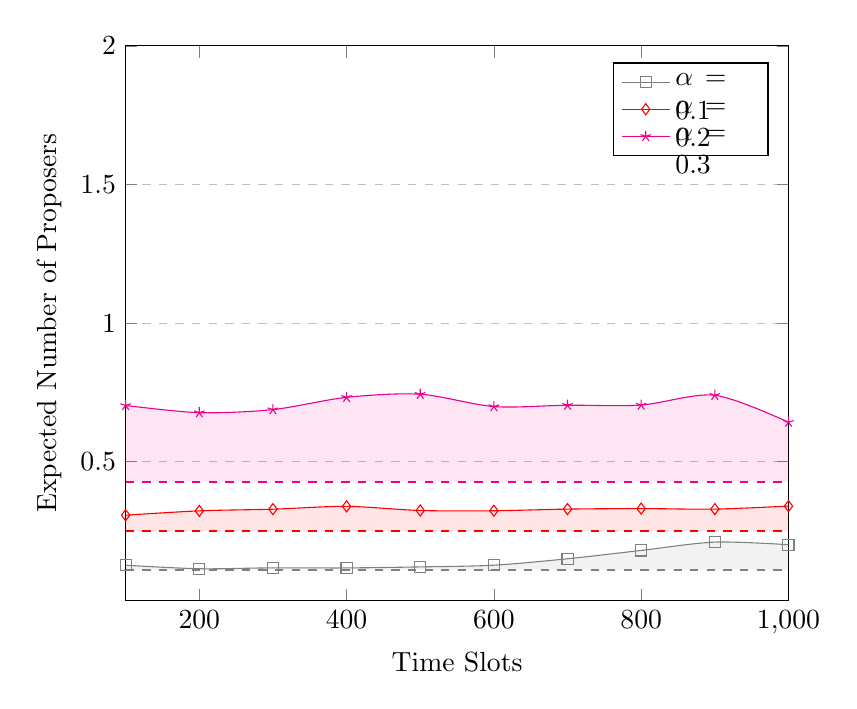
\begin{tikzpicture}
\begin{axis}[
    title={},
    xlabel={Time Slots}, % ($\times 100$},
    ylabel={Expected Number of Proposers},
    xmin=100, xmax=1000,
    ymin=0.0, ymax=2.0,
    xtick={200,400,600,800,1000},
    ytick={0.5,1.0,1.5,2.0},
    legend pos=north east,
    ymajorgrids=true,
    grid style=dashed,
]

\addplot[
	smooth,
    name path=f01,
    color=gray,
    mark=square,
    ]
    coordinates {
(100.0 ,0.1269)
(200.0 ,0.1142)
 (300.0 ,0.1175)
(400.0 ,0.1172)
 (500.0 ,0.1209)
(600.0 ,0.1270)
 (700.0 ,0.1502)
 (800.0 ,0.1803)
 (900.0 ,0.2103)
(1000.0 ,0.2009)
    };
    \addlegendentry[text width=1cm]{$\alpha = 0.1$}
\draw[gray,dashed,thick] (axis cs:100, 0.1111) -- (axis cs:1000, 0.1111);
\path[name path=b01] (axis cs:100, 0.1111) -- (axis cs:1000, 0.1111);

    \addplot [
        thick,
        color=gray,
        fill=gray, 
        fill opacity=0.1,
        forget plot
    ]
    fill between[
        of=f01 and b01,
        soft clip second={domain=100:1000}
    ];
    
\addplot[
	smooth,
    name path=f02,
    color=red,
    mark=diamond,
    ]
    coordinates {
(100.0 ,0.3073)
(200.0 ,0.3230)
(300.0 ,0.3290)
(400.0 ,0.3392)
(500.0 ,0.3243)
(600.0 ,0.3233)
(700.0 ,0.3293)
 (800.0 ,0.3312) 	%
 (900.0 ,0.3293)	%
 (1000.0 ,0.3401)	%
    };
    \addlegendentry[text width=1cm]{$\alpha = 0.2$}
\draw[red,dashed,thick] (axis cs:100, 0.2499) -- (axis cs:1000, 0.2499);
\path[name path=b02] (axis cs:100, 0.2499) -- (axis cs:1000, 0.2499);

    \addplot [
        thick,
        color=red,
        fill=red, 
        fill opacity=0.1,
        forget plot
    ]
    fill between[
        of=f02 and b02,
        soft clip second={domain=100:1000}
    ];
    
\addplot[
	smooth,
    name path=f03,
    color=magenta,
    mark=star,
    ]
    coordinates {
(100.0 ,0.7031)
(200.0 ,0.6770)
(300.0 ,0.6881)
(400.0 ,0.7324)
(500.0 ,0.7436)
(600.0 ,0.6991)
(700.0 ,0.7039)
(800.0 ,0.7045)
(900.0 ,0.7399)
(1000.0 ,0.6426)
    };
    \addlegendentry[text width=1cm]{$\alpha = 0.3$}
\draw[magenta,dashed,thick] (axis cs:100, 0.4284) -- (axis cs:1000, 0.4284);
\path[name path=b03] (axis cs:100, 0.4284) -- (axis cs:1000, 0.4284);

    \addplot [
        thick,
        color=magenta,
        fill=magenta, 
        fill opacity=0.1,
        forget plot
    ]
    fill between[
        of=f03 and b03,
        soft clip second={domain=100:1000}
    ];
    
%\addplot[
%	smooth,
%    color=blue,
%    mark=+,
%    ]
%    coordinates {
%(10.0 ,0)
%(50.0 ,0)
%(100.0 ,0)
%(500.0 ,0)
%(1000.0 ,0)
%    };
%    \addlegendentry[text width=1cm]{$\alpha = 0.4$}
%
%\addplot[
%	smooth, tension=0.2,
%    color=brown,
%    mark=pentagon,
%    ]
%    coordinates {
%(10.0 ,0)
%(50.0 ,0)
%(100.0 ,0)
%(500.0 ,0)
%(1000.0 ,0)
%    };
%    \addlegendentry[text width=1cm]{$\alpha = 0.5$}

%\addplot[
%	smooth, tension=0.2,
%    color=cyan,
%    mark=*,
%    ]
%    coordinates {
%(1 ,0.0000)
%(5 ,0.7879)
%(10 ,0.8540)
%(15 ,0.8807)
%(20 ,0.9077)
%(25 ,0.9253)
%(30 ,0.9356)
%(35 ,0.9497)
%(40 ,0.9619)
%(45 ,0.9648)
%(50 ,1.0000)
%    };
%    \addlegendentry[text width=1cm]{AG}


\end{axis}
\end{tikzpicture}
}
		\label{chr:lws_sf1_10x500}} \\
	\subfloat[][LWS (SF1, 10x1000)]{
		\resizebox{0.4\textwidth}{!}{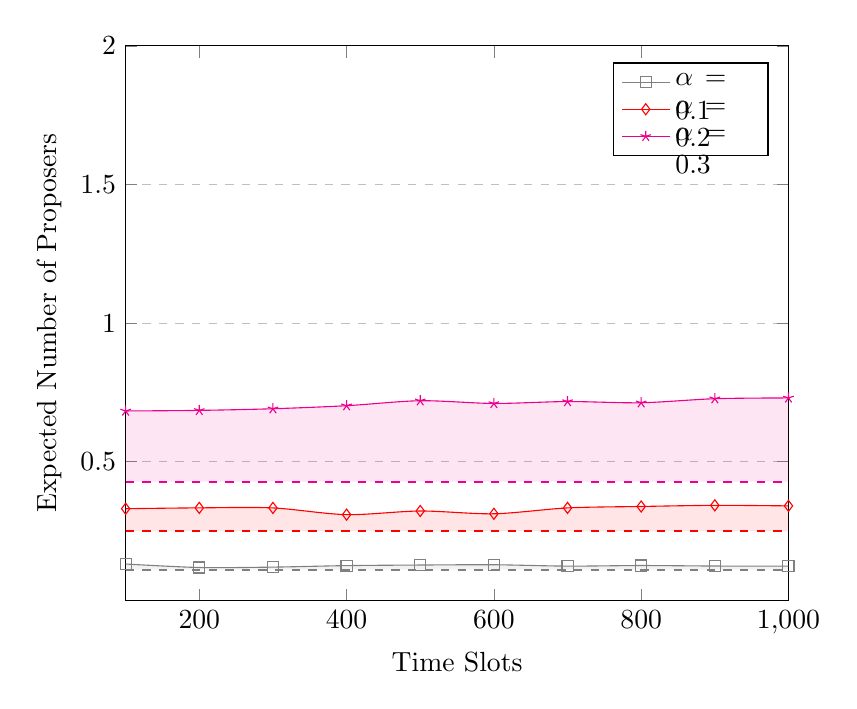
\begin{tikzpicture}
\begin{axis}[
    title={},
    xlabel={Time Slots}, % ($\times 100$},
    ylabel={Expected Number of Proposers},
    xmin=100, xmax=1000,
    ymin=0.0, ymax=2.0,
    xtick={200,400,600,800,1000},
    ytick={0.5,1.0,1.5,2.0},
    legend pos=north east,
    ymajorgrids=true,
    grid style=dashed,
]

\addplot[
	smooth,
     name path=f01,
    color=gray,
    mark=square,
    ]
    coordinates {
(100.0 ,0.1313)
(200.0 ,0.1187)
 (300.0 ,0.1201)
(400.0 ,0.1255)
 (500.0 ,0.1276)
(600.0 ,0.1286)
 (700.0 ,0.1237)
 (800.0 ,0.1258)
 (900.0 ,0.1240)
(1000.0 ,0.1236)
    };
    \addlegendentry[text width=1cm]{$\alpha = 0.1$}
\draw[gray,dashed,thick] (axis cs:100, 0.1111) -- (axis cs:1000, 0.1111);
\path[name path=b01] (axis cs:100, 0.1111) -- (axis cs:1000, 0.1111);

    \addplot [
        thick,
        color=gray,
        fill=gray, 
        fill opacity=0.1,
        forget plot
    ]
    fill between[
        of=f01 and b01,
        soft clip second={domain=100:1000}
    ];
    
    
\addplot[
	smooth,
    name path=f02,
    color=red,
    mark=diamond,
    ]
    coordinates {
(100.0 ,0.3307)
(200.0 ,0.3338)
(300.0 ,0.3336)
(400.0 ,0.3093)
(500.0 ,0.3225)
(600.0 ,0.3124)
(700.0 ,0.3336)		%
 (800.0 ,0.3388) 	%
 (900.0 ,0.3429)	%
 (1000.0 ,0.3409)	%
    };
    \addlegendentry[text width=1cm]{$\alpha = 0.2$}
\draw[red,dashed,thick] (axis cs:100, 0.2499) -- (axis cs:1000, 0.2499);
\path[name path=b02] (axis cs:100, 0.2499) -- (axis cs:1000, 0.2499);

    \addplot [
        thick,
        color=red,
        fill=red, 
        fill opacity=0.1,
        forget plot
    ]
    fill between[
        of=f02 and b02,
        soft clip second={domain=100:1000}
    ];
    
\addplot[
	smooth,
    name path=f03,
    color=magenta,
    mark=star,
    ]
    coordinates {
(100.0 ,0.6832)
(200.0 ,0.6853)
(300.0 ,0.6912)
(400.0 ,0.7022)
(500.0 ,0.7201)
(600.0 ,0.7103)
(700.0 ,0.7172)
(800.0 ,0.7128)
(900.0 ,0.7274)
(1000.0 ,0.7302)
    };
    \addlegendentry[text width=1cm]{$\alpha = 0.3$}
\draw[magenta,dashed,thick] (axis cs:100, 0.4284) -- (axis cs:1000, 0.4284);
\path[name path=b03] (axis cs:100, 0.4284) -- (axis cs:1000, 0.4284);

    \addplot [
        thick,
        color=magenta,
        fill=magenta, 
        fill opacity=0.1,
        forget plot
    ]
    fill between[
        of=f03 and b03,
        soft clip second={domain=100:1000}
    ];
    
%\addplot[
%	smooth,
%    color=blue,
%    mark=+,
%    ]
%    coordinates {
%(10.0 ,0)
%(50.0 ,0)
%(100.0 ,0)
%(500.0 ,0)
%(1000.0 ,0)
%    };
%    \addlegendentry[text width=1cm]{$\alpha = 0.4$}
%
%\addplot[
%	smooth, tension=0.2,
%    color=brown,
%    mark=pentagon,
%    ]
%    coordinates {
%(10.0 ,0)
%(50.0 ,0)
%(100.0 ,0)
%(500.0 ,0)
%(1000.0 ,0)
%    };
%    \addlegendentry[text width=1cm]{$\alpha = 0.5$}
%
%\addplot[
%	smooth, tension=0.2,
%    color=cyan,
%    mark=*,
%    ]
%    coordinates {
%(1 ,0.0000)
%(5 ,0.7879)
%(10 ,0.8540)
%(15 ,0.8807)
%(20 ,0.9077)
%(25 ,0.9253)
%(30 ,0.9356)
%(35 ,0.9497)
%(40 ,0.9619)
%(45 ,0.9648)
%(50 ,1.0000)
%    };
%    \addlegendentry[text width=1cm]{AG}


\end{axis}
\end{tikzpicture}
}
		\label{chr:lws_10x1000}}
	\caption{The expected number of attacker-controlled proposers in the proposers list against execution time in time slots, assuming the attacker is attempting to maximize the length of the compromised tail (\texttt{\#SCORE-FUNCTION} is $1$). The dashed lines represent the base values (with no active attack) computed using Equation~(\ref{eqn:ex_lws}). The shaded areas visualize the expected bias achievable by the attacker for the three different attack probabilities plotted. We assume a proposers list of size $10$, and a validator set of size (a) $10\times 500$ and (b) $10\times 1000$.}
	\label{chr:lws_sf1}
\end{figure}


%\secton{Related Work}

\section{Conclusion}
\label{sec:concl}

We presented an executable formalization of the commit-reveal RANDAO scheme for decentralized random number generation in distributed systems, as a probabilistic rewrite theory in rewriting logic. The theory gives an expressive and executable formal model of the scheme that captures timing of events, probabilistic transitions, environment uncertainties and attacker behaviors. Through its specification in \textsc{Maude}, we used the model to analyze resilience of RANDAO against pre-computed reveal strategies by defining two quantitative measures of achievable bias: the matching score (MS) and the last-word score (LWS), specified as temporal properties in QuaTEx and analyzed using statistical model checking and quantitative analysis with \textsc{PVeSt}A. The analysis described two attack strategies for each property and compared their effectiveness under various assumptions and attack levels. 

This work is still preliminary in that the model enables further kinds of analyses that have not yet been attempted given the time allocated for it. Further analysis could consider scenarios with higher attack probabilities, larger proposer lists and longer execution periods. Moreover, examining how dynamic validator sets, unreliable communication media and extended network latency might affect these attack strategies is all enabled by the model and is interesting to investigate. Furthermore, the analysis presented does not explicitly quantify the costs to the attacker, which can be an important economic defense against mounting these reveal strategies. An extension of the model could keep track of the number of skips, or specify a limit on these skips, so that the success of an attack strategy can be made relative to the cost of executing it. Finally, a holistic approach to analyzing quantitative properties of Serenity looking into availability and attack resilience properties makes for an interesting longer-term research direction.     




%
%\section{Conclusion} 
%\label{sec:conc}
%

\begin{acks}	
We thank Danny Ryan and Justin Drake from the Ethereum Foundation for their very helpful comments. This work was performed under the first Ethereum Foundation security grant ``Casper formal verification''\cite{EFGrants03:2018}.
\end{acks}

%%%%%%%%%%%%%%%%
\bibliographystyle{ACM-Reference-Format}
\bibliography{rdao-report}

%\appendix
%
%\clearpage
%
%



\end{document}
